%Version 3.1 December 2024
% See section 11 of the User Manual for version history
%
%%%%%%%%%%%%%%%%%%%%%%%%%%%%%%%%%%%%%%%%%%%%%%%%%%%%%%%%%%%%%%%%%%%%%%
%%                                                                 %%
%% Springer Nature LaTeX template (sn-article.tex), filled with    %%
%% the manuscript on 14 November 2026.                             %%
%% Class file: sn-jnl.cls, unmodified.                             %%
%%                                                                 %%
%%%%%%%%%%%%%%%%%%%%%%%%%%%%%%%%%%%%%%%%%%%%%%%%%%%%%%%%%%%%%%%%%%%%%%

%% lineno: line numbers in the margin; sn-nature: style for Nature Portfolio journals
\documentclass[lineno,pdflatex,sn-nature]{sn-jnl}% Style for submissions to Nature Portfolio journals

%%%% Standard Packages
%%<additional latex packages if required can be included here>

\usepackage{graphicx}%
\usepackage{multirow}%
\usepackage{amsmath,amssymb,amsfonts}%
\usepackage{amsthm}%
\usepackage{mathrsfs}%
\usepackage[title]{appendix}%
\usepackage{xcolor}%
\usepackage{textcomp}%
\usepackage{manyfoot}%
\usepackage{booktabs}%
\usepackage{algorithm}%
\usepackage{algorithmicx}%
\usepackage{algpseudocode}%
\usepackage{listings}%
\usepackage{bm}% additional package required by this manuscript (bold math symbols)
%%%%

\theoremstyle{thmstyleone}%
\newtheorem{theorem}{Theorem}%
\newtheorem{proposition}[theorem]{Proposition}%

\theoremstyle{thmstyletwo}%
\newtheorem{example}{Example}%
\newtheorem{remark}{Remark}%

\theoremstyle{thmstylethree}%
\newtheorem{definition}{Definition}%

\raggedbottom
\unnumbered% unnumbered level heads, as in Nature Portfolio journals
%% The journal's formatting guidelines ask for references numbered in square brackets.
\setcitestyle{numbers,square,comma,sort&compress}
%% Figures are found either beside this file (single-directory upload) or in figures/ (Overleaf project).


\begin{document}

\title[Resonant enhancement and source priors in subwavelength acoustic reconstruction]{Resonant enhancement and source priors shape subwavelength acoustic reconstruction}

\author[1,3]{\fnm{Nurtugan} \sur{Rysmambetov}}

\author[2,3]{\fnm{Zhanat} \sur{Kappassov}}

%% TO CONFIRM (authors): corresponding author and e-mail address.
\author*[1,3]{\fnm{Bakhtiyar} \sur{Orazbayev}}\email{bakhtiyar.orazbayev@nu.edu.kz}

\affil[1]{\orgdiv{Department of Physics}, \orgname{Nazarbayev University}, \orgaddress{\city{Astana}, \country{Kazakhstan}}}

\affil[2]{\orgdiv{School of Computing and Artificial Intelligence}, \orgname{Nazarbayev University}, \orgaddress{\city{Astana}, \country{Kazakhstan}}}

\affil[3]{\orgdiv{Robotics Center}, \orgname{Institute of Smart Systems and Artificial Intelligence, Nazarbayev University}, \orgaddress{\city{Astana}, \country{Kazakhstan}}}

\abstract{Resonant metalenses promise acoustic imaging below the diffraction limit, a long-standing goal. However, subwavelength images reflect both measured waves and assumptions about the source. Here we develop and experimentally test a calibrated framework that distinguishes these two contributions. Combining a coupled-resonator model with measurements on an eight-source array, we compare detection, known-profile amplitude estimation, and unknown-profile recovery. We demonstrate that precise amplitude estimates can coexist with substantial profile distortion: for the finest recorded pattern, the metalens reduces the median amplitude error from $7.3\%$ to $2.1\%$, while the five-record root-mean-square (RMS) relative profile error falls from $0.94$ to $0.63$ under rank-five truncated inversion. The model shows why: detection and amplitude estimation use the whole received response, whereas profile recovery also depends on weak source directions and noise amplification during inversion. The metalens changes the gains and spatial structure of these directions, so its benefit depends on the source pattern. Specifically, under the stated noise model and full-profile RMS-error criterion, the calculated relative reconstruction requirements decrease by $17.0$~dB for a sine but $1.2$~dB for a cosine at the same spatial frequency. Moreover, by varying priors at fixed recordings, we show how compatible assumptions improve recovery and incorrect assumptions introduce false structure. Priors constrain weakly determined source components, and both effects are smaller with the metalens in the measured two-source comparison. Our findings show where subwavelength images are determined by measurement and where by source assumptions, providing a quantitative basis for designing and validating ultrasonic and other wave-based imagers.}

\keywords{acoustic metamaterials, resonant metalens, subwavelength imaging, inverse problems, source priors}

\maketitle

\section{Introduction}

A central difficulty in far-field subwavelength acoustic imaging is that sources with different fine features can produce nearly identical recordings. This is because fine spatial variations excite evanescent components that rapidly decay away from the source. In near-field acoustic holography, it is possible to access these components by measuring close to the radiating surface~\cite{maynard1985,williams1999}. However, at distant sensors, the response can instead be dominated by features shared by several source profiles. Therefore, the total signal may therefore be strong even when the differences needed to recover fine features are obscured by noise~\cite{kim2003}. While regularization limits noise amplification during inversion, it can also suppress source detail~\cite{williams2001,hansen2010}. Thus, assessing a recovered image requires examining two stages: how the waves encode source differences and how the reconstruction uses the recorded information.

The recent development of resonant metalenses allowed to modify the first stage by coupling to fields near the source and changing how they reach distant sensors. Such near-field scatterers and coupled resonator arrays have enabled subwavelength focusing in microwaves and sound~\cite{lerosey2007,lemoult2010,lemoult2011prl}. In these resonator arrays, fine spatial structure can be encoded into frequency-dependent radiated responses. Moreover, for Helmholtz resonators, the link between resonance and time-reversal super-resolution has also been established mathematically~\cite{ammari2015}. In locally-resonant metamaterials, collective coupling and multiple scattering can enhance transmission and produce acoustic superlensing~\cite{yang2015,kaina2015}, while cavity resonances support evanescent-wave transmission and field enhancement~\cite{zhu2011,cheng2013,chen2021,yuan2021}. Other approaches combine spatial mixing with joint-sparsity reconstruction through blind structured illumination in airborne sound and near-field scattering in ultrasound~\cite{lin2022blind,lin2025blind}. These approaches illustrate how physical encoding and reconstruction constraints can work together, making the assumptions used during decoding part of the imaging method.

The second stage is decoding the sensor recordings into a source profile. When several profiles remain compatible with noisy data, source priors guide this inference by specifying which profiles are more plausible. They change the inference from the data without changing the measured response. Traditional Bayesian methods express source knowledge through probability distributions and covariance assumptions~\cite{antoni2012,stuart2010,pereira2015,caviedes2021}, while sparse methods favor a few active expansion coefficients or equivalent sources~\cite{chardon2012,fernandez2017}. Another approach, based on mathematical super-resolution, guarantees likewise dependendancy on assumptions about sparsity and separation~\cite{donoho1992,candes2014}, and combining sparsity with resonant encoding can also support subwavelength imaging~\cite{mu2022}. Finally, recent rise of neural decoders~\cite{arridge2019,fernandez2023} demonstrated that learned empirical priors can also regularize acoustic inversion~\cite{lobato2024}. In our earlier work, we combined deep learning with a lossy acoustic metalens to reconstruct and recognize features as small as $\lambda/30$~\cite{orazbayev2020}.

These source assumptions matter most when different profiles produce similar recordings. Compatible priors can improve recovery, whereas incorrect ones can introduce false structure~\cite{bhadra2021,gottschling2025}. Moreover, learned reconstructions can also miss structural changes or be sensitive to small perturbations~\cite{antun2020}. And a reconstructed image alone does not establish how strongly its features are constrained by the measurements. More importantly, the information required also depends on the task and on what is already known about the source. Therefore, there are three main tasks for the decoder: (i) detection, (ii) estimation and (iii) reconstruction. Detection asks whether a response can be distinguished from noise. Estimating the amplitude of a known profile leaves only one complex scale unknown, while recovering an unknown profile requires estimating its spatial coefficients. Thus, detectable signals and precise amplitude estimates can  coexist with uncertainty about the source shape. This is supported by the previous works on noise-dependent resolution in microwave imaging, which further illustrate the need to specify measurement conditions~\cite{davy2009}.

To compare these three tasks, we need a common physical description, which is provided by a linear transfer operator~\cite{prada1994,miller2000}. We calculate this operator from the forward model and determine it experimentally through calibration measurements with known source drives~\cite{tanter2000,popoff2010}. Its singular-value decomposition then identifies orthogonal source patterns and the gains with which they reach the sensors~\cite{aubry2010,miller2019}. By using such spatially encoded acoustic measurements, we can illustrate how distinct responses can support subwavelength reconstruction~\cite{tian2022}. For instance, for a specified source profile, the relevant information depends on how it projects onto these patterns, not only on the strongest response or the number of retained channels. Whereas weak transmission of one component can limit recovery even when other components produce a strong signal~\cite{hansen2010}. And adding a lens can change both the gains and the source patterns themselves. Therefore, a stated noise model and recovery criterion are needed to compare measurement requirements and to ask how changes in physical encoding differ from changes in source assumptions.

Here we show that what a resonant metalens adds to subwavelength acoustic imaging depends on the recovery task and on the source pattern, and that its contribution can be distinguished experimentally from that of source priors. We develop and experimentally test a framework that separately quantifies how resonant enhancement and source priors shape subwavelength reconstruction. Combining a coupled-resonator model with calibrated measurements on an eight-source acoustic array, we compare detection, known-profile amplitude estimation and unknown-profile recovery under fixed task criteria. We demonstrate, using separately acquired source recordings, that precise amplitude estimates can coexist with substantial profile distortion. Moreover, for sine and cosine patterns with the same half-period of $\lambda/13$, calculations on the measured operators give relative reconstruction-budget reductions of $17.0$ and $1.2$~dB under the stated noise model and full-profile RMS-error criterion. Therefore, the lens benefit depends on which source pattern is encoded, even at a fixed spatial scale. And by varying priors at fixed recordings, we then isolate improvements from compatible assumptions and false structure introduced by incorrect ones. We demonstrate that in the measured two-source comparison, both effects are smaller with the lens, showing that stronger physical encoding can reduce dependence on source knowledge. These controlled comparisons provide a quantitative basis for assessing what a resonant imager contributes to a specified reconstruction task and can be used to assess whether other wave-based imaging systems are limited by the physical measurement or by source knowledge.


\section{Results}

\subsection{Detection does not establish profile recovery}
First, we start with a coupled-resonator model to show why strong recordings need not distinguish different source profiles, see Fig.~\ref{fig:pair} (more details in Methods). In this model, eight driven acoustic sources couple to a nearby metalens of ten resonators, and six far-field microphones sample the combined field radiated by the sources and the lens. We write the recording as $\mathbf y=T\mathbf a+\mathbf n$, where $\mathbf a$ contains the eight dimensionless relative source-drive coefficients, $T$ maps them to stacked microphone--frequency samples, and $\mathbf n$ is recording noise. These coefficients specify the prescribed drives and the model separately solves for the amplitudes developed by the interacting radiators. In the model, we use the reference wavelength $\lambda_0$ at the lens resonance, with $\lambda=\lambda_0$ in pattern labels.

To identify the source patterns and their transmission gains, we use the singular-value decomposition (SVD), $T=U\Sigma V^\dagger$. Each eight-component unit source vector $v_i$ produces a unit recording vector $u_i$ multiplied by its gain: $Tv_i=\sigma_i u_i$. The columns of $U,V$ collect these recording and source vectors, $\Sigma$ contains the gains on its diagonal, and $\dagger$ denotes conjugate transpose. Moreover, we order the gains from strongest to weakest, so the index of $v_i$ identifies an SVD direction rather than an individual radiator. For the two-profile comparison below, we restrict the drives to real values and obtain the source vectors from the SVD of $[\operatorname{Re}T;\operatorname{Im}T]$, which stacks the real and imaginary observations.

Then, by using the strongest and weakest real-source singular vectors of the no-lens operator, we construct the unit-norm profiles $s_1=(v_1+v_8)/\sqrt2$ and $s_2=(v_1-v_8)/\sqrt2$ (Fig.~\ref{fig:pair}a). The profiles share the same $v_1$ component and differ only in the sign of $v_8$. As expected, their common component can produce a detectable recording even when the weak response that distinguishes them is obscured by noise. We keep these two profiles fixed when adding the lens and use the same absolute noise level in both conditions. Moreover, we assume independent zero-mean complex Gaussian noise with equal real and imaginary variances $\sigma_n^2/2$, giving $\mathbb E|n_j|^2=\sigma_n^2$ per sample. Figure~\ref{fig:pair}(b) shows the field difference $\Delta p=p(s_1)-p(s_2)$, where $p(s_i)$ is the model acoustic field of candidate $s_i$. To quantify distinguishability, we project the recordings onto the direction of the difference between the two predicted recordings (Fig.~\ref{fig:pair}c). Their mean separation, measured in units of the noise standard deviation in this projection, is only $0.0087$ without the lens, compared with $83.66$ with it. Thus, the lens makes these two specified profiles distinguishable by strengthening the recorded difference between them. Supplementary Notes 1--6 give the model assumptions and physical controls.


\begin{figure}[!t]
\centering
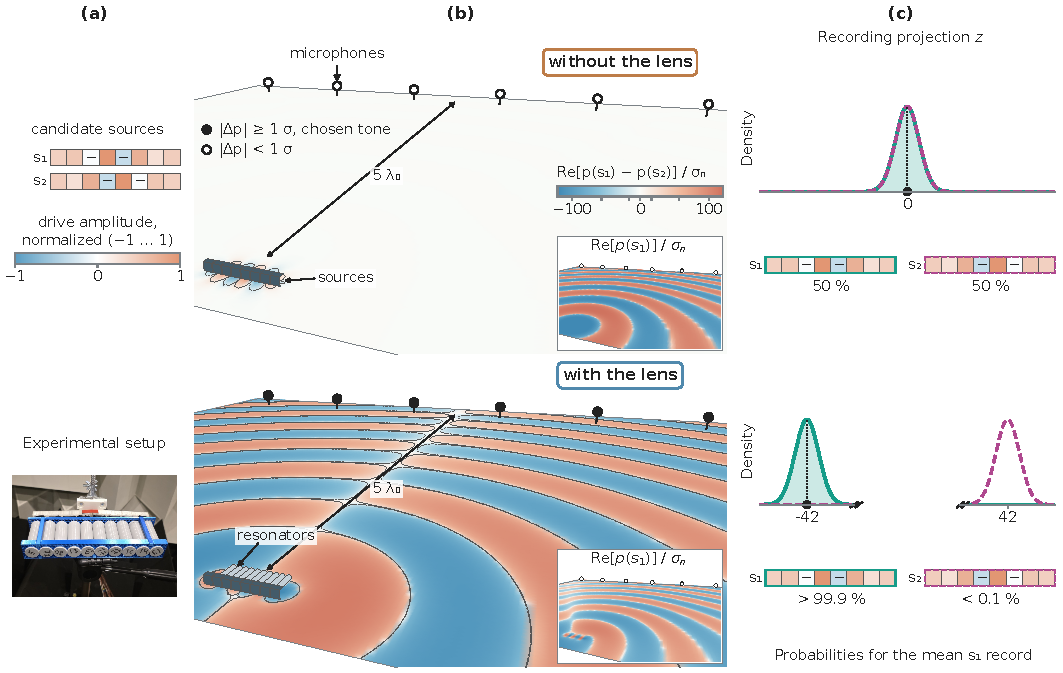
\includegraphics[width=\textwidth]{figures/main/current/Fig1.pdf}
\caption{}\label{fig:pair}
\end{figure}

In the preceding example, the possible source profiles are specified in advance. We now ask whether a recording that supports precise amplitude estimation for a known profile also supports recovery when its shape is not supplied. Figure~\ref{fig:model} compares these tasks for three model patterns. For a known unit-norm profile $\phi$, we write $\mathbf a=A\phi$ and fit its predicted response $AT\phi$ to the recording. Therefore, only the common complex multiplier $A$, which sets the overall amplitude and phase, is unknown. For unknown-profile recovery, the estimator is given the transfer operator $T$ but not the shape $\phi$: it must infer all eight complex source-drive coefficients from the recording.

Recovering these coefficients requires undoing the different transmission gains of the source directions. Dividing by a small gain also amplifies recording noise. We therefore use truncated singular-value decomposition (TSVD), which reconstructs the source from the $r$ retained singular directions,
\begin{equation}
 \hat{\mathbf a}=\sum_{i=1}^{r}\frac{u_i^\dagger\mathbf y}{\sigma_i}\,v_i,
 \label{eq:tsvd}
\end{equation}
where $r$ is the retained channel count. Each term estimates the source component along $v_i$ by projecting the recording onto $u_i$ and dividing by $\sigma_i$. Discarding weak channels limits noise amplification, but also removes any true source components along those directions.

To assess the accuracy of this reconstruction, we use the root-mean-square (RMS) relative profile error,
\begin{equation}
 E_{\rm prof}=\left[\frac{\mathbb E\|\hat{\mathbf a}-\mathbf a\|^2}{\|\mathbf a\|^2}\right]^{1/2}.
 \label{eq:profile_rms}
\end{equation}
Here $\|\cdot\|$ is the Euclidean norm and the expectation averages over the assumed recording noise. All eight complex source coefficients contribute to the error, without refitting a common amplitude or phase. We require $E_{\rm prof}\le1/\sqrt2$, corresponding to at least a factor-of-two reduction in mean-square error relative to the zero reconstruction $\hat{\mathbf a}=0$. We choose this threshold as a performance benchmark and report continuous errors and tolerance sensitivity alongside the pass/fail comparisons.

Consequently, we apply the comparison to three unit-norm model profiles: the $\lambda/5$ cosine, $\lambda/10$ sine and $\lambda/20$ cosine, where the labels specify spatial half-periods (Fig.~\ref{fig:model}). The coupled-resonator model uses a coarser source array than the acoustic bench to illustrate the mechanism (Methods). Moreover, we set the illustrative reference budget to $B=20\log_{10}(\sigma_1/\sigma_n)=64$~dB. Each lens condition uses its own strongest singular gain $\sigma_1$ to set the noise level, so equal budgets do not imply equal absolute noise; this model budget is not calibrated to the bench. Detection requires the received pattern power to exceed the total recording noise power. Therefore, for known-profile amplitude estimation, we require an RMS error of at most $4\%$ for the complex multiplier $A$, with true $A=1$.

At this budget, all three profiles meet the detection and known-profile amplitude criteria (Fig.~\ref{fig:model}a,b). For unknown-profile recovery, only the coarsest $\lambda/5$ cosine passes the full-profile error criterion without the lens, whereas all three profiles pass with it (Fig.~\ref{fig:model}c). Specifically, the finest pattern, the $\lambda/20$ cosine, provides the clearest contrast: without the lens, the scalar fit has an RMS amplitude error of only $0.70\%$, while the RMS relative profile error is $0.98$. Remarkably, adding the lens reduces the latter to $0.024$.

Futhermore, at the chosen reference budget, the spectral rule specified in Methods retains three complex singular channels without the lens and all eight with it. The profile pass/fail outcomes remain unchanged throughout the sampled $62.0$--$75.4$~dB range, showing that the contrast between amplitude precision and profile recovery persists beyond the single $64$~dB setting. Supplementary Note 7 gives the noise-budget and tolerance-sensitivity checks.


\begin{figure}[!t]
\centering
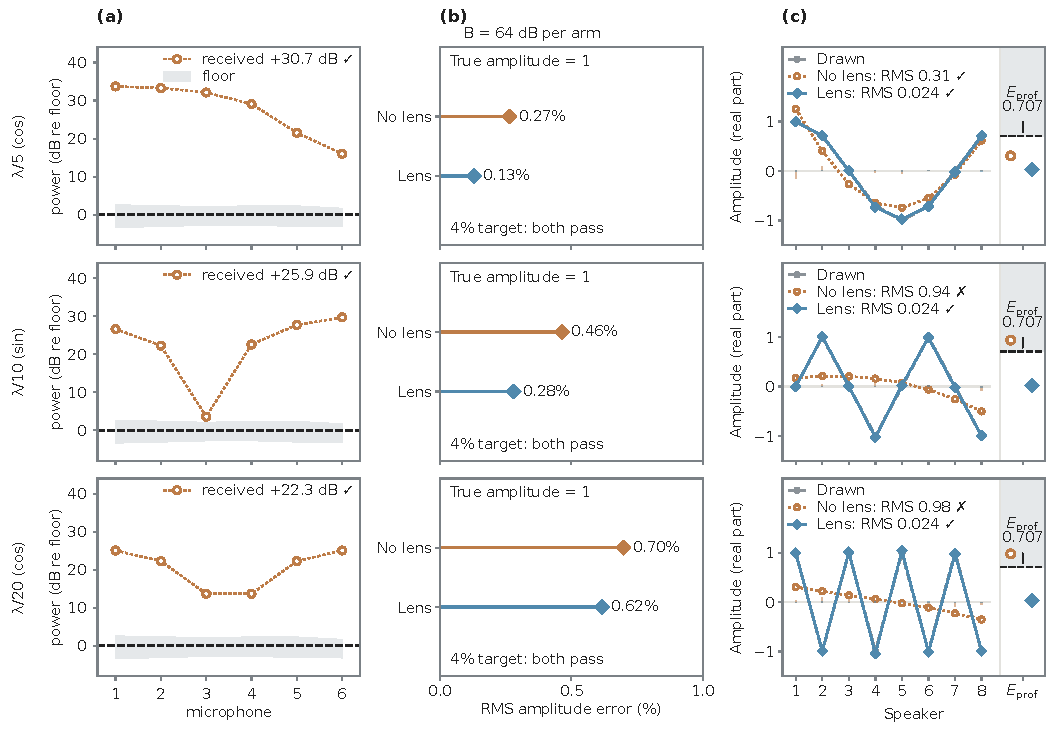
\includegraphics[width=\textwidth]{figures/main/current/Fig2.pdf}
\caption{}\label{fig:model}
\end{figure}

\subsection{The lens improves recorded source profiles}
We next experimentally examine the lens effect on an acoustic bench with eight loudspeakers at $0.038\lambda_0$ pitch, ten Helmholtz resonators and six far-field microphones. We measure each loudspeaker separately and stack the microphone responses over $350$--$450$~Hz to form a calibrated transfer operator (Methods). Our experimental analysis has two stages: (i) we calculate task-specific requirements on the measured operators under a stated noise model (Fig.~\ref{fig:budget}b--d), alongside recorded driven-pattern powers (Fig.~\ref{fig:budget}a); (ii) we then test reconstruction directly using source recordings acquired separately from calibration (Fig.~\ref{fig:recorded}).

The eight source-drive profiles in Figure~\ref{fig:budget} form the real Fourier basis of the array: a uniform profile, three sine--cosine pairs and an alternating cosine, where the pattern labels specify spatial half-periods. Here the direct comparison in Figure~\ref{fig:recorded} uses three separately recorded profiles: the $\lambda/6.5$ sine, $\lambda/13$ sine and $\lambda/26$ cosine.

Furthermore, for the budget analysis, we obtain the baseline-normalized operator $T$ by dividing each microphone--frequency row of the calibrated operator by the standard deviation of its source-off baseline recordings. However, this scaling does not remove correlations and an additional assumption about the amplitude and reconstruction calculations is made by using independent proper-complex Gaussian noise. Finally, we select complex singular channels using the floor rule: a channel is retained when its singular value exceeds a threshold proportional to the assumed noise level (Methods). The retained rank therefore changes as that level is varied.

Thus, at the acquired background level, this rule retains $3/4/3$ complex channels for the initial no-lens, with-lens and repeat no-lens sessions. Adding the lens raises the fourth singular value from $12.9$ to $79.7$, taking it across the selection threshold, while the strongest value rises from $395$ to $789$. It should be noted that the fourth gain increases more in relative terms. Overall, these gains describe ordered singular directions: the same index need not represent the same spatial profile in the two operators. Moreover, a supplementary control applies the relative cutoff $0.03\sigma_1$ before baseline normalization and retains $4/5/4$ channels, with $\sigma_1$ defined for that unweighted operator (Supplementary Note 10 and Supplementary Fig.~6). Supplementary Notes 8--12 and Supplementary Figs.~5--7 give the apparatus, calibration and repeatability controls.

At equal drive norms, the finer $\lambda/19.5$ cosine gives recorded power levels of $11.84$~dB without the lens and $25.46$~dB with it; the coarser $\lambda/13$ cosine gives $13.79$ and $20.56$~dB, respectively (Fig.~\ref{fig:budget}a). These levels are relative to each condition's background power. Adding the lens therefore reverses which of these two patterns gives the stronger response at the sampled microphones.

However, these power measurements alone do not establish whether the source profiles can be recovered. We therefore compare the relative budgets required for detection, known-profile amplitude estimation and unknown-profile recovery. To do so, we vary the assumed noise level on the measured operators for each unit-norm pattern (Fig.~\ref{fig:budget}b--d). Each condition's budget is referenced to the strongest singular gain of its baseline-normalized operator. However, detection and known-pattern amplitude fitting use different statistics and tolerances, so their required budgets do not define a universal ranking of task difficulty. For profile recovery, we use the same full-profile criterion $E_{\rm prof}\le1/\sqrt2$. Here the prescribed shape is used only to score the TSVD output. Each required budget is the lowest sampled value from which the task criterion remains satisfied as the assumed noise is reduced. Thus, the acquired-background lines provide reference budgets under the diagonal noise model, not empirically validated recovery margins. Supplementary Note 16 examines background correlations using a separate estimator.

At the acquired background level, $6$ of eight patterns pass the $4\%$ amplitude tolerance without the lens and all $8$ pass with it. For profile recovery, $3$ of eight patterns pass without the lens and $4$ with it. Moreover, all $16$ plotted recovery thresholds coincide, on the sampled budget grid, with a channel entering the retained subspace under the floor rule.

Interestingly, the calculated reconstruction-budget change depends on the spatial pattern, even at a common spatial frequency. For instance, at a half-period of $\lambda/13$, the saving is $1.2$~dB for the cosine and $17.0$~dB for the sine. For the $\lambda/19.5$ sine, the required budget instead rises from $69.1$ to $70.7$~dB with the lens. However, these changes describe relative requirements under the stated reconstruction rule, not absolute noise margins.

Moreover, the chosen profile-error tolerance also affects these savings. For the finest $\lambda/26$ cosine, tightening the RMS tolerance from $1/\sqrt2$ to $0.5$ changes the calculated budget saving from $12.3$ to $2.3$~dB (Supplementary Note 7). The same stricter tolerance reverses the $\lambda/13$ cosine's budget advantage, while preserving the full-profile error definition.


\begin{figure}[!t]
\centering
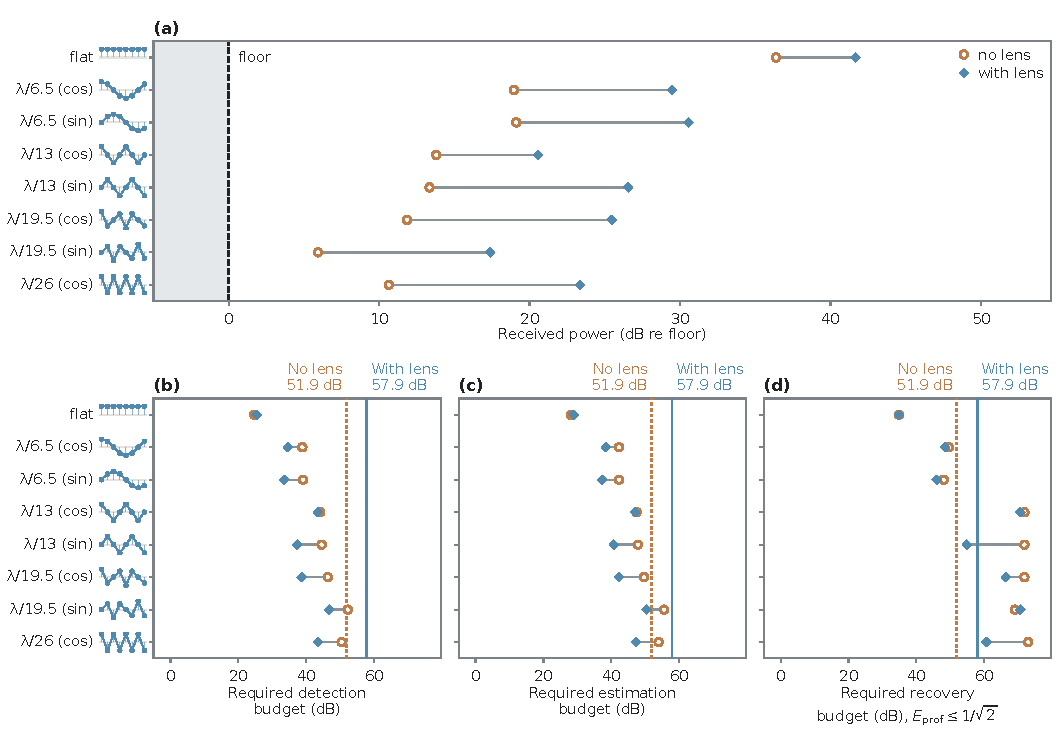
\includegraphics[width=\textwidth]{figures/main/current/Fig3.pdf}
\caption{}\label{fig:budget}
\end{figure}

We next test reconstruction directly on source recordings acquired separately from calibration (Fig.~\ref{fig:recorded}). For unknown-profile recovery, we fix the complex TSVD rank at five in both lens conditions and derive the reconstruction weights from the magnitudes of the first source-off baseline recording in each condition (Methods); these rank and weighting choices do not enter the known-profile amplitude fit. For the alternating $33$~mm pattern, labelled $\lambda/26$, the median error of the known-profile complex amplitude fit falls from $7.3\%$ without the lens to $2.1\%$ with it across five recordings. The full-profile RMS relative error falls from $0.94$ to $0.63$, with squared relative errors averaged across all five complex reconstructions before taking the square root and without amplitude or phase refitting. Therefore, at the common threshold, $0/3$ no-lens cases and $3/3$ with-lens cases pass. Fig.~\ref{fig:recorded}c displays the first reconstruction for each case. Here the finest with-lens profile still has substantial distortion despite passing the chosen tolerance.

Figure~\ref{fig:recorded}(b) also compares the observed scalar errors with the conditional amplitude-error bound $\epsilon/g$. For the prescribed drive $\mathbf a_0$, we define $g=\|H\mathbf a_0\|$ and assume that $\epsilon=0.03\sigma_1(H)\|\mathbf a_0\|$ bounds the norm of the complete recording error. Here $H$ is the drive-scaled calibrated operator before row weighting, and $\sigma_1(H)$ is its strongest singular value. The $3\%$ scale is motivated by median recording prediction errors, which include calibration mismatch; these medians do not establish a bound for every recording. The plotted limits are conditional on this assumed bound, rather than measured error bars or confidence intervals.

Consequently, reprocessing the same recordings shows that these pass/fail counts depend on the chosen rank and weighting. For instance, at rank four, the finest with-lens profile has an RMS relative error of $0.84$ for the first set of weights and fails the tolerance for all nine sets. The coarsest no-lens profile passes at rank four for all nine weightings and, at rank five, for six of the nine (Supplementary Note 11 and Supplementary Table 1). The comparison therefore demonstrates improvement at a matched rank, without establishing rank-independent resolution of the finest pattern. Supplementary Fig.~7 provides additional repeatability comparisons with separately phase-aligned and peak-normalized profile displays.


\begin{figure}[!t]
\centering
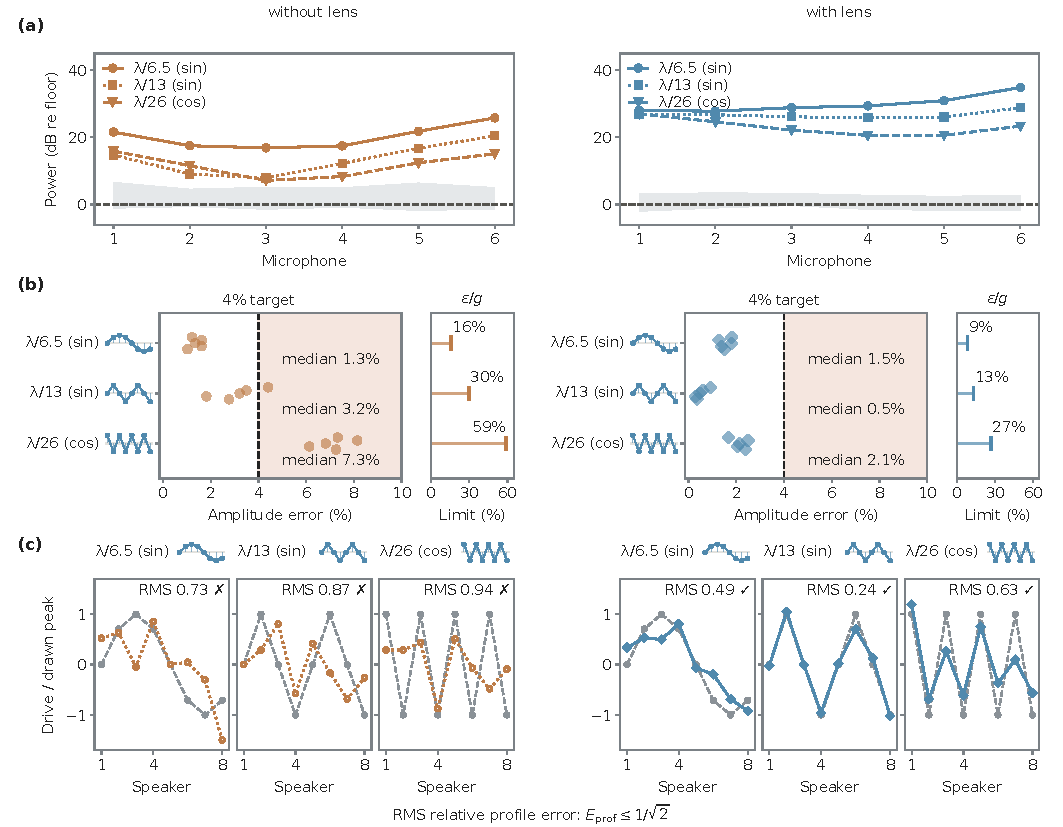
\includegraphics[width=\textwidth]{figures/main/current/Fig4.pdf}
\caption{}\label{fig:recorded}
\end{figure}

\subsection{Source assumptions can improve or distort reconstruction}
Having compared reconstruction with and without the metalens, we now isolate the effect of source assumptions. To do so, we hold the recording and transfer operator fixed within each lens condition and compare estimates with no additional source prior, with a compatible prior and with an incorrect prior (Fig.~\ref{fig:prior}). For more visual demonstration, we first examine a controlled two-coefficient model and then apply the same comparison to separately recorded acoustic profiles.

To this end, we first illustrate the comparison with two unknown real coefficients multiplying the fixed with-lens reference patterns $v_3,v_5$, using the same physical patterns and priors in both lens conditions. We choose an illustrative relative budget of $24$~dB, at which the source prior visibly affects the estimate. At this budget, we take the true coefficients to be $(1,1)$ and compare zero-mean Gaussian priors with unit marginal variances and correlations $\pm0.9$. Thus, the $+0.9$ prior is compatible with this source because it favors coefficients of the same sign, whereas the $-0.9$ prior favours opposite signs and imposes an incorrect relationship. For the fixed recording in each condition, the compatible prior improves the estimate, while the incorrect prior increases its error. We then train a neural decoder for each operator and prior on independent simulated examples. The outputs show the same qualitative effects as the Gaussian posterior-mean estimate (Methods), illustrating how source assumptions learned during training can improve or distort reconstruction.

We then apply this comparison to a separately recorded profile driven at speakers one and three. Here the priors express assumptions about which source positions are likely to be active: the compatible prior favours positions one and three, whereas the incorrect prior favours one and two. Both are soft constraints, so all eight real source coefficients remain free. Using the same data within each lens condition, we compare the resulting profiles with the data-only estimate. Without the lens, the relative profile errors for the data-only, compatible-prior and incorrect-prior estimates are $21.0\%$, $5.4\%$ and $58.6\%$, respectively. With the lens, the corresponding errors are $3.9\%$, $3.6\%$ and $22.8\%$. Thus, compatible source knowledge substantially improves the no-lens reconstruction, whereas an incorrect assumption introduces substantial error in either lens condition.

To make this comparison on a common basis, we first average the five recordings of the target profile and use this same averaged recording for all three estimates. To characterize reconstruction error, we separately apply real least squares to the mean recording of each of the other seventeen source profiles and compare the recovered coefficients with the known drive coefficients. From these errors, we estimate an empirical bias and full covariance, with all target recordings excluded from this fit. We then subtract the fitted bias from the target's least-squares estimate to obtain the data-only baseline. Here data only means that no additional source prior is applied: this baseline still uses the calibrated transfer operator and the error calibration obtained from the other profiles. Both prior-based estimates use this same baseline and fitted error covariance. Finally, the axes display coefficients along the fixed no-lens singular patterns $v_5,v_7$, while profile errors use all eight source coefficients.


\begin{samepage}
To visualize this uncertainty, the shaded ellipses in Figure~\ref{fig:prior} describe the estimation error of the data-only baseline in the two displayed coordinates. Each ellipse is centred on the data-only estimate and remains fixed when we change the source prior within a lens condition. By contrast, a posterior region describes uncertainty in the source coefficients after combining the recording with a specified prior. Let $\mathbf x$ contain the two displayed coefficients, $\mathbf x_{\rm data}$ their data-only estimate and $S_{\rm view}$ its error covariance. The shaded region is
\begin{equation}
 \label{eq:uncertainty}
 \mathcal U_2=\{\mathbf x\in\mathbb R^2:(\mathbf x-\mathbf x_{\rm data})^{\mathsf T}S_{\rm view}^{-1}(\mathbf x-\mathbf x_{\rm data})\le4\}.
\end{equation}
Its principal semiaxes are twice the square roots of the covariance eigenvalues, so a longer direction marks a combination of coefficients that the data constrain less. In the model, the covariance follows from the assumed Gaussian recording noise (Methods). For the measured example, $S_{\rm view}$ is the submatrix for directions five and seven of the full empirical coefficient-error covariance. Thus, under an exact zero-mean two-dimensional Gaussian estimation-error law, such radius-two regions contain the true displayed coefficients in $86.5\%$ of repeated realizations, rather than $95\%$. For the measured contour, however, this error law is a working description with no established coverage for arbitrary sources.
\end{samepage}

With the lens, the data constrain the relevant source components more strongly in these examples. Consequently, a compatible prior provides less additional improvement, while an incorrect prior produces a smaller increase in profile error, relative to the data-only baseline in each lens condition. The arrow labels quantify these changes in relative profile error in percentage points (pp), without assigning each image feature uniquely to data or assumptions. Supplementary Notes 13--15 give the general Gaussian channel weights, prior-coordinate transformations and a separate model coefficient control with different reference patterns and priors; Supplementary Fig.~8 shows the model and measured source singular patterns.


\begin{figure}[!t]
\centering
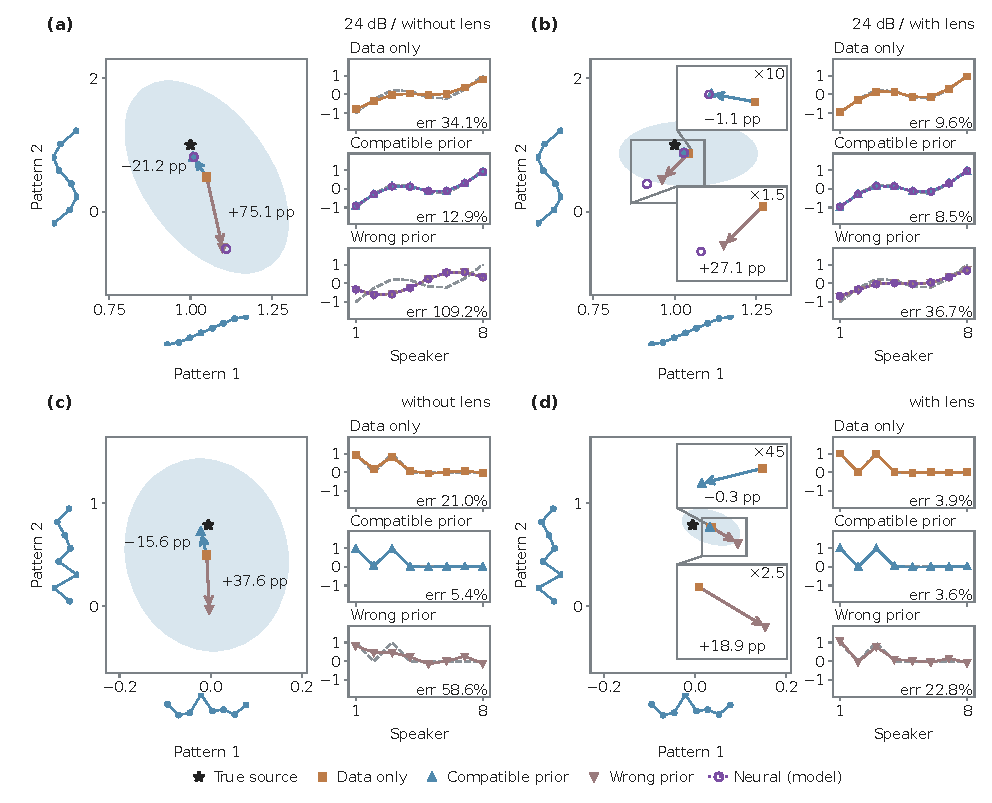
\includegraphics[width=\textwidth]{figures/main/current/Fig5.pdf}
\caption{}\label{fig:prior}
\end{figure}

\section{Discussion}

In this work, by building on resonant subwavelength encoding~\cite{lemoult2010,lemoult2011prl}, learned metalens imaging~\cite{orazbayev2020} and sparse resonant reconstruction~\cite{mu2022}, we extend these demonstrations with a controlled assessment of how physical encoding and source assumptions contribute to a specified recovery task. By varying the lens under fixed reconstruction rules and varying priors at fixed recordings within each lens condition, we make these contributions separately testable in the same calibrated system. Moreover, combining these controls with three explicit tasks and separately acquired source profiles, we distinguish gains in signal strength and amplitude precision from gains in spatial fidelity.

First, we demonstrate with separately acquired recordings that precise amplitude estimates can coexist with substantial profile distortion. Supplying the source shape removes spatial ambiguities from the estimation task, so a precise amplitude fit does not show that the recording resolves those ambiguities. Consequently, amplitude precision and spatial fidelity should be evaluated separately, with the latter assessed from the full-profile error when the shape is not supplied to the estimator. A demonstrated feature size then describes performance for the tested profiles and estimator, rather than a universal resolution boundary.

Moreover, our calibrated operators show that the lens benefit depends on how each source pattern is encoded. A source pattern is a combination of singular source directions, and weak transmission of its components makes their recovery sensitive to noise~\cite{kim2003}. Therefore, the number of retained channels alone does not determine recovery: their gains and the pattern's projections also matter. Because the lens changes both the gains and the directions themselves, it can benefit two patterns differently even at the same spatial frequency. For instance, for the sine and cosine with half-period $\lambda/13$, we quantify this difference as reductions of $17.0$ and $1.2$~dB in the calculated relative reconstruction requirements under the stated noise model, inversion rule and full-profile RMS-error criterion. These budgets are referenced to each operator's strongest singular gain, so they compare relative requirements rather than absolute noise margins. Since resonator geometry and dispersion shape propagation and focusing~\cite{lanoy2021,kingsley2022}, the same analysis can compare candidate geometries and acquisition bands according to how well they support recovery of an intended source class.

In turn, the role of weakly constrained source components helps explain how physical encoding affects the influence of source priors. A prior can guide their reconstruction by favoring particular coefficient relationships or active positions. Such source knowledge also enters Bayesian acoustic focusing, which can adapt the source aperture and its distribution jointly~\cite{antoni2019}. To isolate this contribution, we compare compatible and incorrect priors while holding the recording and operator fixed within each lens condition. With the lens, the data constrain the relevant components more strongly in our model and recorded pair. Consequently, the compatible prior provides less additional improvement and the incorrect prior introduces a smaller increase in error relative to the data-only baseline. Moreover, the neural decoders in the two-coefficient model reproduce these qualitative effects when trained on independent simulated examples under the same priors. Thus, stronger physical encoding can improve recovery while also reducing its dependence on a source description that may be wrong.

These conclusions are based on one eight-source acoustic array and one lens installation for the main recorded recovery comparison, so repeated recordings characterize variation within this setting. The prescribed drives are real, while the profile inverse allows complex coefficients and the prior comparisons restrict them to real values. Thus, neither comparison tests arbitrary-phase sources. In addition, the illustrative model uses a coarser two-dimensional array with assumed driver and loss parameters. Its omission of out-of-plane propagation limits its representation of the apparatus, since such propagation can affect Helmholtz-resonator focusing~\cite{basham2024}, and forward-model uncertainty can alter acoustic inverses~\cite{gilquin2019}. Moreover, the quantitative requirements depend on the assumptions used in the analysis: the calculated budgets treat the calibrated operators as known and assume normalized white noise, while the $3\%$ complete-error bound and the measured-prior Gaussian error law remain working assumptions without validation for arbitrary sources. The amplitude tolerance, matched reconstruction rank and floor cutoff were also selected retrospectively, without a separate threshold-selection test set. Consequently, the reported pass/fail outcomes must be read together with the stated rank, weighting and error criterion. Thus, these experimental and analytical conditions limit transfer of the numerical results to other installations and source distributions.

Nevertheless, our framework provides a quantitative basis for deciding which source components need stronger physical encoding and where reliable source knowledge can improve recovery. This links choices of hardware, acquisition settings and reconstruction priors to measurable performance for the intended source class. To apply the approach in another system, we must calibrate its linear transfer operator, specify the source class, error model and recovery criterion, and validate the resulting comparisons on separately acquired source profiles. With those conditions established, the approach could guide the design and assessment of ultrasonic arrays, non-destructive-testing probes and other calibrated imaging platforms.

\section{Methods}

\subsection{Bench and lens}

Eight loudspeakers at $33$~mm pitch $d$ form the source array and drive a lens of ten cylindrical Helmholtz resonators. At $400$~Hz, $\lambda_0\simeq858$~mm, so the pitch is $0.038\lambda_0$. Here $\lambda_0=c/f_0$ is the reference wavelength, with sound speed $c=343$~m~s$^{-1}$ and reference frequency $f_0=400$~Hz. The Fourier aperture convention is $L=8d=264$~mm; the distance between the outer source centres is $7d=231$~mm. Each resonator is a closed cavity with a coaxial neck, printed in one piece by fused deposition. In the recorded lens installation, the ten resonators are spaced at $23$~mm, with the lens and source-array centres aligned. The caliper-recorded throat-to-speaker-line gap readings span $0$--$2$~mm (Supplementary Note 8). Twenty-one resonators were characterized as side branches on a four-microphone impedance tube by the two-source method (ASTM International standard E2611). Their recorded resonance frequencies span $394.5$--$404.5$~Hz with mean $400.2$~Hz. Supplementary Fig.~5 identifies the ten mounted elements (Supplementary Note 9). Twelve laser range measurements determine the six microphone positions. Five lie on an arc of radius approximately $2.455$~m and one at $2.00$~m, over an angular span of $61.5^\circ$ (Supplementary Note 10). The main recorded recovery comparison uses one lens installation.


\subsection{Source excitation and data acquisition}

The acquisition sequence is an initial measurement without the lens, a measurement with the lens installed, and a repeat after removing it. We stack $41$ tones over $350$--$450$~Hz for each condition at the nominal $0.10$~V drive setting. We write the electrical drive as $\mathbf d(f)=s(f)\mathbf a$, where $s(f)$ is the common complex tone phasor in volts, $f$ is frequency and $\mathbf a$ contains dimensionless relative drive coefficients. The magnitude and phase of $s(f)$ specify the sinusoidal excitation. Each loudspeaker plays in phase or in antiphase with the common tone, so the driven coefficients are real. One drive unit is the calibration drive. Microphone data are in output units, not calibrated to pascals.


Calibrations average nine single-speaker recordings per column. Five recordings of each test pattern are retained separately. The initial no-lens and with-lens measurements each hold nine baseline (no-excitation) recordings; the repeat after lens removal uses the with-lens baseline. The reduced export contains $90$ separate image, flat and staggered recordings per session. The additional sine-pattern phasors used in Figure~\ref{fig:recorded} were extracted from the original recordings with the frozen fast Fourier transform (FFT) convention; acquisition identifiers and hashes accompany them. The reduced exports retain the averaged calibration, rather than the individual calibration time series (Supplementary Note 8). Recordings sharing a calibration or baseline are technical repeats, not independent lens installations (Supplementary Notes 11--12).


\subsection{Stacked operator noise and rank rules}

For each tone, we form $H$ from the mean of nine single-speaker calibration recordings and subtract the baseline mean. It has six microphone rows and eight speaker columns. We keep the calibration drive in $H$, without dividing by the drive phasor, and stack all tones. In the local per-volt convention, $H_V(f)=Y_{\rm cal}^{\mathsf T}(D_{\rm cal}^{\mathsf T})^+$. Multiplying by the tone phasor gives the same drive-scaled calibration, $H(f)=s(f)H_V(f)$. Rows of $Y_{\rm cal}$ and $D_{\rm cal}$ contain the microphone and electrical drive phasors for each calibration; $\mathsf T$ is transpose and $+$ the Moore--Penrose pseudoinverse. Thus $H_V$ has microphone-output units per volt, whereas $H$ includes one calibration drive. The calibrated relation is $\mathbf y=H\mathbf a+\mathbf e$, with complete recording error $\mathbf e$.


For Figure~\ref{fig:budget}, we estimate the baseline standard deviation from nine baseline recordings. The indices $k,m,j$ denote tone, microphone and source, respectively. The value $\sigma_{km}$ describes one tone and microphone, using deviations about the baseline mean and sample-variance denominator eight. It describes the noise of one recording, with the convention $\mathbb E|n_{km}|^2=\sigma_{km}^2$, rather than the standard error of a mean. Dividing each row by $\sigma_{km}$ gives the dimensionless complex stack $T_{km,j}=H_{km,j}/\sigma_{km}$; this row normalization is the baseline weighting used here. It standardizes marginal variances but does not remove cross-sample correlations. Independent proper-complex Gaussian noise after normalization is an additional assumption of the amplitude and recovery budget calculations~\cite{schreier2010}.


The complex floor-rank rule retains singular values above the operational cutoff $3(\sqrt{KM}+\sqrt N)=55.54$ at $\sigma_n=1$, with $K=41$ tones, $M=6$ microphones and $N=8$ sources. The multiplier three places the truncation above the dimension-dependent reference scale $\sqrt{KM}+\sqrt N$; its role is to limit inversion of weak channels. Testing multipliers two and four leaves the paired budget savings unchanged within one grid step (Supplementary Note 7). This cutoff is a conservative operational truncation rule, not a measured detection boundary or a confidence threshold. Floor rank is the number of singular values above this cutoff at a given budget. A hard rank instead specifies the truncation directly; Figure~\ref{fig:recorded} uses five in both arms. For the relative budget defined in Results, $\sigma_1$ is the top singular value of the arm's baseline-normalized complex stack, and $\sigma_n=1$ at the acquired background level. The budget needed is the lowest sampled budget above which the criterion continues to hold as the noise scale is reduced. The matched complex channel count and floor rule were chosen after acquisition; scalar fits and fixed-prior examples are retrospective analyses of acquired data. Since each arm has its own $\sigma_1$, a common relative budget need not mean equal absolute error.


For eight arbitrary complex source coefficients, a single-tone six-microphone operator has rank at most six. Restricting the coefficients to real values gives twelve real observations, so counting alone does not exclude recovery; conditioning, the sensitivity of the inverse to recording errors, remains decisive. A separate supplementary control uses the empirical relative spectral cutoff $0.03\sigma_1$ without row normalization. It gives counts $4/5/4$ for the initial no-lens, with-lens and repeat no-lens measurements, respectively, whereas Figure~\ref{fig:budget}'s matched complex rule gives $3/4/3$. The rules use different error conventions on the same recordings (Supplementary Note 10). For this control, $\sigma_1$ refers to the drive-scaled $H$. With $\hat{\mathbf y}$ formed by stacking $H(f)\mathbf a=H_V(f)\mathbf d(f)$, we report the recording prediction error, $\|\mathbf y-\hat{\mathbf y}\|/(\sigma_1\|\mathbf a\|)$. It includes calibration mismatch and is not a per-sample noise standard deviation. Median recording prediction errors are $2.89\%$, $1.76\%$ and $3.14\%$ for the initial no-lens, with-lens and repeat no-lens measurements, respectively. They motivate the selected $3\%$ scale used for the conditional complete-error bound in Figure~\ref{fig:recorded}(b), but establish neither a bound on every recording nor a noise standard deviation.


The baseline-weighted operator described above uses the baseline standard deviations. The recorded reconstructions use separate weight arrays derived from the magnitudes of individual baseline recordings. For the first array, $W_{(km),(km)}=1/|b^{(1)}_{km}|$, where $b^{(1)}_{km}$ is the first source-off recording at tone $k$ and microphone $m$, without subtraction of the baseline mean. These arrays provide weights, rather than noise estimates. To display the profiles in Figure~\ref{fig:recorded}, we use the first weight array and first driven recording of the frozen complex-return export, with the mean calibration operator. The single displayed profiles use neither repeat aggregation nor individual calibration operators. Figure~\ref{fig:recorded}(b) reports all five acquired scalar errors and their medians; panel (c) uses the same recording and weighting indices in every cell.


\subsection{Pattern ladder}

We construct the ladder from the real discrete Fourier transform (DFT) of the eight-element array, $\cos(2\pi pj/8)$ and $\sin(2\pi pj/8)$. Here $j=0,\ldots,7$ indexes source position and the integer $p$ indexes spatial frequency; plots number these speakers one to eight. This gives eight patterns: the flat pattern, three cosine--sine pairs and the alternating cosine. Its nonzero wavenumbers are approximately $23.8$, $47.6$, $71.4$ and $95.2$~rad~m$^{-1}$. With Fourier aperture $L=8d$, $k=2\pi p/L$ is the pattern's transverse wavenumber, distinct from the acoustic wavenumber in the coupled-dipole model. The half-period is $\pi/k=L/(2p)$ for nonzero $p$. The coupled-dipole model uses a coarser array, so its rungs have different half-periods from the bench. Scores on driven recordings use the actual peak-one drive $\mathbf a_0$ in drive units. Conditional calculations use the unit-norm pattern $\phi=\mathbf a_0/\|\mathbf a_0\|$. The supplementary type-II discrete cosine transform (DCT-II) probes $\phi_m(j)\propto\cos[\pi m(j+1/2)/8]$, with mode index $m=0,\ldots,7$, form a different basis (Supplementary Note 7).


\subsection{The three criteria}

Total-noise detection compares received pattern power with total recording noise power. For the model in Figure~\ref{fig:model}, these are $\|T\phi\|^2$ and $KM\sigma_n^2$. For Figure~\ref{fig:budget}(b), the comparison precedes row normalization: signal power is $\|H\phi\|^2$ and, at noise multiplier $\sigma_n$, total noise power is $\sigma_n^2\sum_{km}\sigma_{km}^2$. Hence $B_{\rm det}=20\log_{10}[\sigma_1(T)(\sum_{km}\sigma_{km}^2)^{1/2}/\|H\phi\|]$. Panels (c,d) instead use the row-normalized operator $T$. Recorded driven powers are reported separately in their actual drive scale. These conventions specify no false-alarm probability.


For scalar amplitude fitting, the shape $\mathbf a_0$ is known, $\mathbf a=A\mathbf a_0$, and $\mathbf h=H\mathbf a_0$. The unregularized complex fit is
\begin{equation}
 \hat A=\frac{\mathbf h^\dagger\mathbf y}{\mathbf h^\dagger\mathbf h},\qquad g=\|\mathbf h\|.
\end{equation}
True $A=1$. For zero-mean proper-complex white recording error, let $\sigma_{\rm raw}$ be the per-sample standard deviation in microphone-output units. The RMS error is $[\mathbb E|\hat A-1|^2]^{1/2}=\sigma_{\rm raw}/g$: it averages squared error over the assumed noise before taking the square root, without bounding every recording or giving a confidence probability. An explicitly assumed complete recording-error bound $\|\mathbf e\|\leq\epsilon$ instead gives $|\hat A-1|\leq\epsilon/g$. We use a $4\%$ amplitude-error tolerance, $\tau=0.04$, selected retrospectively from the empirical $95$th percentile of five-repeat RMS scalar errors across $58$ pattern--session cases ($290$ recordings; Supplementary Note 7). The percentile is $3.60\%$; rounding upward to the next whole percentage point gives $4\%$. We require $\mathbb E|\hat A-A|^2/|A|^2\le0.0016$ under the stated noise model. Equivalently, the scalar-fit signal-to-noise ratio $g^2/\sigma_{\rm raw}^2$ must be at least $625$ ($27.96$~dB). This is a descriptive precision benchmark, not a measured apparatus threshold. Changing the tolerance to $\tau$ shifts every scalar amplitude budget by $20\log_{10}(0.04/\tau)$; the exact lens--no-lens budget difference is unchanged. Supplementary Note 7 tests $2\%$ and $8\%$ tolerances and gives the corresponding budget shifts and measured-ladder sensitivity. Figure~\ref{fig:recorded} uses $\epsilon=0.03\sigma_1\|\mathbf a_0\|$, with $\sigma_1$ from the drive-scaled $H$; the observed errors are $|\hat A-1|$. The bound is conditional and is not inferred from the five observed errors.


Figure~\ref{fig:budget}(c) uses the same one-amplitude test after baseline normalization: fit $A$ from $T\phi_\ell$ and the normalized recording, with $\|\phi_\ell\|=1$. Here $\ell$ labels an acquired Fourier-ladder pattern, separately from the supplementary DCT-II index $m$. The normalized noise standard deviation is $\sigma_n=1$ at the acquired background level. For $g_\ell=\|T\phi_\ell\|$, the exact budget for RMS amplitude error at most $0.04$ is
\begin{equation}
 B_{\rm amp}(\ell)=20\log_{10}\!\left(\frac{\sigma_1}{0.04g_\ell}\right).
\end{equation}
The plotted mark is the first passing point on the $0.1$~dB grid. All channels enter the scalar fit; no additional prior is imposed on the unknown complex amplitude. Here $\sigma_n$ is a per-sample noise standard deviation, whereas $\epsilon$ in Figure~\ref{fig:recorded} bounds the complete recording error. These are different error conventions for the same known-pattern amplitude task.


\subsection{Estimators}

Acoustic inverse filtering can be expressed through a calibrated propagation matrix~\cite{tanter2000}. For Figure~\ref{fig:recorded}, let $W$ be the diagonal matrix of the individual-baseline weights specified above, and set $\widetilde H=WH$, $\widetilde{\mathbf y}=W\mathbf y$. Apply the TSVD estimator in equation~\eqref{eq:tsvd} to $\widetilde{\mathbf y}$, using the singular vectors and gains of $\widetilde H$~\cite{hansen2010}. The hard rank is five in both arms, with the baseline-weighting protocol specified above applied to all five records. This matches the retained dimension rather than optimizing each arm for the known truth. Fixing the first baseline and driven recording makes the display reproducible without choosing the smallest error; Supplementary Note 11 tests neighbouring ranks and all baseline weights. We score all five returns by the RMS relative profile error in equation~\eqref{eq:profile_rms}, with true drive $\mathbf a_0$, counting the imaginary component and fitting neither amplitude nor phase.


For a unit true pattern $\phi$, let $V_r$ contain the retained source singular vectors and $P_r=V_rV_r^\dagger$ be their orthogonal projector. Under independent proper-complex white recording noise, the full-profile score has the exact form
\begin{equation}
 E_{\rm prof}^2=1-\|P_r\phi\|^2+\sigma_n^2\sum_{i\le r}\sigma_i^{-2}.
 \label{eq:profile_risk}
\end{equation}
The first term measures discarded squared source norm; the sum measures noise amplified across all retained inverse directions. Figures~\ref{fig:model}(c) and \ref{fig:budget}(d) evaluate this noise expectation exactly. Figure~\ref{fig:recorded}(c) estimates the same RMS score from its five complex reconstructions using equation~\eqref{eq:profile_rms}; recording errors there also include calibration mismatch. Its one displayed profile is the first recording, with the fixed weighting specified above. No Gaussian error law is inferred from those five records.


For the budget-dependent reconstruction test in Figure~\ref{fig:budget}(d), apply complex TSVD to $T\phi_\ell+\mathbf n$, retaining singular values $\sigma_i>3(\sqrt{KM}+\sqrt N)\sigma_n$. Evaluate equation~\eqref{eq:profile_risk} at every $0.1$~dB grid point and report the first budget from which $E_{\rm prof}\le1/\sqrt2$ remains satisfied. Increasing rank can introduce a noise-variance jump, so an isolated earlier passing point does not define the required budget. In the noise-free limit, the same profile tolerance reduces to the supplementary capture condition $C_m\geq0.5$ for a unit DCT-II probe, with $C_m=\|P_r\phi_m\|^2$. Reconstruction similarity, $\rho=|\hat{\mathbf a}^\dagger\mathbf a|/(\|\hat{\mathbf a}\|\|\mathbf a\|)$, is reported only in its stated supplementary controls and ignores common scale and phase. Supplementary Note 7 gives the error derivation and tolerance sensitivity; the Gaussian-prior controls in Notes 13--15 use their own stated distributions~\cite{rodgers2000}.


\subsection{Source priors and neural decoders}

For the model in Figure~\ref{fig:prior}, we take directions three and five of one fixed with-lens real-stack SVD basis. Both arms use these same physical patterns and priors at $24$~dB relative budget. The true coefficient vector is $(1,1)$. To form the data-only observation, we add a prescribed error: the lower-triangular Cholesky factor of the least-squares covariance times $(0.4,-0.55)$. We do not search noise draws to select this displacement. The priors are zero-mean Gaussians with unit marginal variances and correlations $+0.9$ or $-0.9$. Unit variance sets the coefficient scale; the opposite correlations impose equally strong, compatible or wrong relations without changing either marginal variance. The $24$~dB budget places this example in a regime where the prior can visibly affect the estimate. For the fixed physical-pattern matrix $\Phi=[v_3,v_5]$, define $T_{\Phi,\rm R}=[\operatorname{Re}(T\Phi);\operatorname{Im}(T\Phi)]$. The data-only coefficient-error covariance is $S_{\rm view}=(\sigma_n^2/2)(T_{\Phi,\rm R}^{\mathsf T}T_{\Phi,\rm R})^{-1}$, using variance $\sigma_n^2/2$ per real observation.


We train a neural decoder for each operator and prior. It takes the sufficient least-squares statistic, the coefficient estimate retaining all coefficient information under the stated Gaussian measurement model, as two standardized inputs and returns two coefficients through a hidden layer of $32$ ReLU units, using the rectified linear unit (ReLU) activation $\max(0,x)$ for scalar input $x$. Training targets are independently sampled true coefficients. We add independent Gaussian observation errors with the same covariance as the analytic model. The Adam stochastic-gradient optimizer minimizes coefficient mean-square error for $8000$ steps with batches of $512$. A cosine schedule lowers the learning rate from $10^{-3}$ to $10^{-5}$. Each of three fixed seeds ($101$, $202$, $303$) is evaluated on $32768$ independent draws; seed $101$ is displayed without selection. Validation compares the network with the exact Gaussian conditional mean under its own training prior, which minimizes expected squared error~\cite{bishop2006}. We evaluate the fixed plotted source separately, including under the mismatched prior. It never supplies a training label. Saved outputs, checkpoints and validation records accompany the figure.


For the measured example, take the mean of all five recordings of the fixed pair at speakers one and three. Real least-squares coefficient errors on the other seventeen recorded source-class means determine a bias and full covariance $S$. Subtract the fitted bias to obtain the data-only statistic $\mathbf z$. A soft zero-mean prior has source-coordinate covariance $C$ with diagonal entries one on the favoured positions and $0.01$ elsewhere. This gives a tenfold standard-deviation contrast, favouring the specified support while leaving all coefficients free; it is a controlled source restriction rather than an estimated source population. Write the real drive as $\mathbf a=V_\star\mathbf c$, where $\mathbf c$ contains dimensionless real coefficients and $V_\star$ is the complete fixed no-lens reference basis. Transform the bias-corrected statistic, prior mean $\bm\mu$, source covariance $C$ and error covariance $S$ into these coordinates, retaining full covariances. In the following update, $\mathbf z$, $\bm\mu$, $C$ and $S$ denote these transformed quantities; the estimate is~\cite{stuart2010}
\begin{equation}
 \hat{\mathbf c}=\bm\mu+C(C+S)^{-1}(\mathbf z-\bm\mu).
\end{equation}
All target records are held out when fitting $S$ and the bias. This is a Gaussian working-error assumption, not a validated distribution for arbitrary sources. The displayed coordinates are directions five and seven of the fixed no-lens real-stack reference basis. Profile errors are calculated from all eight components; arrow labels are changes in those errors in percentage points. Supplementary Note 14 gives the coordinate transformation, preserving induced correlations.


\subsection{Coupled-dipole model}

For Figures~\ref{fig:pair}, \ref{fig:model} and \ref{fig:prior}(a,b), we use a two-dimensional scalar coupled-dipole (Foldy--Lax, or repeated point-scattering) model based on multiple-scattering theory~\cite{foldy1945,lax1951}, following the implementation of ref.~\cite{orazbayev2020}. We solve $A\bm p=\bm e$, where $\bm e=(\mathbf a,\mathbf0)^{\mathsf T}$ applies drives only at the eight sources and $\bm p$ contains the solved complex scatterer amplitudes of sources and resonators. The interaction matrix has off-diagonal entries $A_{jl}=g_fG(kr_{jl})$ and diagonal entries $A_{jj}=g_f[Q_j(f_{0,j}^2-f^2)+i(1+\gamma_j)]$. Here $j,l$ index the sources and resonators, $r_{jl}$ is their separation, $k=2\pi f/c$ is acoustic wavenumber, $i^2=-1$, $g_f=(2\pi f)^2/4$ and $G(kr)=Y_0(kr)+iJ_0(kr)$ is the outgoing two-dimensional Green function for time convention $e^{+i2\pi ft}$. Here $t$ is time and $J_0,Y_0$ are zeroth-order Bessel functions of the first and second kind, respectively. Model lengths and frequencies use units $\lambda_0$ and $f_0$, with sound speed $c=1$; $f_{0,j},Q_j,\gamma_j$ specify each element's resonance, resonant self-term coefficient and absorption relative to radiation damping. The transfer operator is $T(f)=-g_fG_{\rm mic}A^{-1}|_{\rm source}$. $G_{\rm mic}$ propagates from every scatterer to the microphones; the restriction keeps source-drive columns. Each source and resonator is a point scatterer with a resonant response. This approximation does not represent the full three-dimensional acoustic geometry. Source drives are distinct from the solved scatterer amplitudes.


Lens elements resonate at $f_0$. Model parameters are $Q=16$, lens absorption $\gamma=0.02$, source resonance $0.9f_0$, source self-term coefficient $0.7$ and absorption $4$. The quality-factor scale is motivated by isolated-resonator validation (Supplementary Note 9). The lens loss specifies a weak-absorption reference, while the source parameters specify broad, strongly damped drivers. Supplementary Note 1 quantifies these choices and their sensitivity; they do not fit the installed lens or measured loudspeaker impedances. Twenty tones span $0.8$--$1.2f_0$. The source pitch is $0.05\lambda_0$ and the lens standoff is $0.4d$. Both arrays are centred at $y=0$. The ten lens elements are equally spaced on a parallel line from $y=-0.15\lambda_0$ to $y=0.15\lambda_0$, giving half-height $3d$ and pitch $2d/3$. Six microphones span $\pm3\lambda_0$ on a line at $5\lambda_0$. For Figure~\ref{fig:model}, the floor rule uses $K=20$, $M=6$, $N=8$ and retains three complex no-lens channels. The noise is proper-complex white, with $\mathbb E|n_j|^2=\sigma_n^2$ per complex sample. Figure~\ref{fig:model} uses $64$~dB relative to each operator's own strongest singular value. For a unit-norm drive, this gives the per-sample noise-to-gain ratio $\sigma_n/\sigma_1=10^{-64/20}\simeq6.31\times10^{-4}$; it is neither the received-signal SNR nor a measured experimental noise level. Figure~\ref{fig:pair} uses the common absolute noise of the no-lens reference budget. The model illustrates the questions with a coarser array than the bench; it does not fit the bench. Supplementary Notes 1--6 give the physical assumptions and controls; supporting literature for the supplementary derivations is listed in Supplementary References.


For the two-candidate example, write $\mathbf y_i=Ts_i$, $\Delta\mathbf y=\mathbf y_2-\mathbf y_1$ and $\bar{\mathbf y}=(\mathbf y_1+\mathbf y_2)/2$. The recording projection is
\begin{equation}
 z=\frac{\operatorname{Re}[\Delta\mathbf y^\dagger(\mathbf y-\bar{\mathbf y})]}{(\sigma_n/\sqrt2)\|\Delta\mathbf y\|},\quad
 d=\frac{\sqrt2\|\Delta\mathbf y\|}{\sigma_n}.
\end{equation}
Here $z$ and the separation $d$ in Figure~\ref{fig:pair}(c) are dimensionless; this $d$ differs from the source pitch used elsewhere. $\mathcal N(\mu,\sigma^2)$ denotes a real Gaussian with mean $\mu$ and variance $\sigma^2$. Thus $z|s_1\sim\mathcal N(-d/2,1)$ and $z|s_2\sim\mathcal N(d/2,1)$. Equal initial candidate probabilities give $P(s_1|\mathbf y_1)=[1+\exp(-d^2/2)]^{-1}$. This probability at a mean recording differs from average binary classification error.

\backmatter

% Treat back-matter headings as top-level PDF bookmarks.
\makeatletter
\def\toclevel@subparagraph{1}
\makeatother

\bmhead{Supplementary information}

Supplementary Notes 1--16, Supplementary Figs.~1--8 and Supplementary Table 1 accompany this article.

\bmhead{Data availability}

The experimental measurements and numerical data generated using our custom simulation code are archived in Zenodo at \url{https://doi.org/10.5281/zenodo.24221204} (version 1.0.0)~\cite{rysmambetov2026data}. The archive includes reduced measurements, calibration operators, background recordings, frozen model and figure inputs, numerical outputs, trained-network checkpoints and selected raw waveforms. Source Data for the main figures are provided with this paper and in the archive. Other raw time series are available from the corresponding author on reasonable request.

\bmhead{Code availability}

The custom simulation, reconstruction, neural-network training, figure-generation and numerical-verification code is archived with the data in Zenodo at \url{https://doi.org/10.5281/zenodo.24221204} (version 1.0.0) and is available under the MIT licence. The repository is maintained at \url{https://github.com/wavelabnu/acoustic-metalens-source-recovery}. SHA-256 checksums identify the archived inputs and code; the neural-network records include training distributions, random seeds and operator fingerprints.

\bmhead{Author contributions}

N.R. and B.O. designed the study. B.O. built the measurement setup and wrote the acquisition and analysis code. B.O. and Z.K. performed the experiments. N.R. developed the coupled-resonator model, characterized the resonators, and carried out the simulations. B.O. and N.R. analyzed the data. B.O. and Z.K. acquired funding. B.O. and Z.K. supervised the project. All authors discussed the results and wrote the manuscript.


\bmhead{Funding}

This research was funded by the Science Committee of the Ministry of Science and Higher Education of the Republic of Kazakhstan (Grant No. AP26195569), by Nazarbayev University under FDCRGP no 040225FD4719.

\bmhead{Competing interests}

The authors declare no competing interests.

\begin{thebibliography}{10}
\expandafter\ifx\csname url\endcsname\relax
  \def\url#1{\burl{#1}}\fi
\expandafter\ifx\csname urlprefix\endcsname\relax\def\urlprefix{URL }\fi
\providecommand{\bibinfo}[2]{#2}
\providecommand{\eprint}[2][]{\url{#2}}
\providecommand{\doi}[1]{\url{https://doi.org/#1}}
\bibcommenthead

\bibitem{maynard1985}
\bibinfo{author}{Maynard, J.~D.}, \bibinfo{author}{Williams, E.~G.} \&
  \bibinfo{author}{Lee, Y.}
\newblock \bibinfo{title}{Nearfield acoustic holography: {I}. Theory of
  generalized holography and the development of {NAH}}.
\newblock \emph{\bibinfo{journal}{Journal of the Acoustical Society of
  America}} \textbf{\bibinfo{volume}{78}}, \bibinfo{pages}{1395--1413}
  (\bibinfo{year}{1985}).
\newblock \doi{10.1121/1.392911}.

\bibitem{williams1999}
\bibinfo{author}{Williams, E.~G.}
\newblock \emph{\bibinfo{title}{Fourier Acoustics: Sound Radiation and
  Nearfield Acoustical Holography}}  (\bibinfo{publisher}{Academic Press},
  \bibinfo{address}{London}, \bibinfo{year}{1999}).
\newblock \doi{10.1016/B978-0-12-753960-7.X5000-1}.

\bibitem{kim2003}
\bibinfo{author}{Kim, Y.} \& \bibinfo{author}{Nelson, P.~A.}
\newblock \bibinfo{title}{Spatial resolution limits for the reconstruction of
  acoustic source strength by inverse methods}.
\newblock \emph{\bibinfo{journal}{Journal of Sound and Vibration}}
  \textbf{\bibinfo{volume}{265}}, \bibinfo{pages}{583--608}
  (\bibinfo{year}{2003}).
\newblock \doi{10.1016/S0022-460X(02)01452-9}.

\bibitem{williams2001}
\bibinfo{author}{Williams, E.~G.}
\newblock \bibinfo{title}{Regularization methods for near-field acoustical
  holography}.
\newblock \emph{\bibinfo{journal}{Journal of the Acoustical Society of
  America}} \textbf{\bibinfo{volume}{110}}, \bibinfo{pages}{1976--1988}
  (\bibinfo{year}{2001}).
\newblock \doi{10.1121/1.1404381}.

\bibitem{hansen2010}
\bibinfo{author}{Hansen, P.~C.}
\newblock \emph{\bibinfo{title}{Discrete Inverse Problems: Insight and Algorithms}}
  (\bibinfo{publisher}{SIAM}, \bibinfo{address}{Philadelphia}, \bibinfo{year}{2010}).
\newblock \doi{10.1137/1.9780898718836}.

\bibitem{lerosey2007}
\bibinfo{author}{Lerosey, G.}, \bibinfo{author}{de~Rosny, J.},
  \bibinfo{author}{Tourin, A.} \& \bibinfo{author}{Fink, M.}
\newblock \bibinfo{title}{Focusing beyond the diffraction limit with far-field
  time reversal}.
\newblock \emph{\bibinfo{journal}{Science}} \textbf{\bibinfo{volume}{315}},
  \bibinfo{pages}{1120--1122} (\bibinfo{year}{2007}).
\newblock \doi{10.1126/science.1134824}.

\bibitem{lemoult2010}
\bibinfo{author}{Lemoult, F.}, \bibinfo{author}{Lerosey, G.},
  \bibinfo{author}{de~Rosny, J.} \& \bibinfo{author}{Fink, M.}
\newblock \bibinfo{title}{Resonant metalenses for breaking the diffraction
  barrier}.
\newblock \emph{\bibinfo{journal}{Physical Review Letters}}
  \textbf{\bibinfo{volume}{104}}, \bibinfo{pages}{203901}
  (\bibinfo{year}{2010}).
\newblock \doi{10.1103/PhysRevLett.104.203901}.

\bibitem{lemoult2011prl}
\bibinfo{author}{Lemoult, F.}, \bibinfo{author}{Fink, M.} \&
  \bibinfo{author}{Lerosey, G.}
\newblock \bibinfo{title}{Acoustic resonators for far-field control of sound on
  a subwavelength scale}.
\newblock \emph{\bibinfo{journal}{Physical Review Letters}}
  \textbf{\bibinfo{volume}{107}}, \bibinfo{pages}{064301}
  (\bibinfo{year}{2011}).
\newblock \doi{10.1103/PhysRevLett.107.064301}.

\bibitem{ammari2015}
\bibinfo{author}{Ammari, H.} \& \bibinfo{author}{Zhang, H.}
\newblock \bibinfo{title}{A mathematical theory of super-resolution by using a
  system of sub-wavelength {Helmholtz} resonators}.
\newblock \emph{\bibinfo{journal}{Communications in Mathematical Physics}}
  \textbf{\bibinfo{volume}{337}}, \bibinfo{pages}{379--428}
  (\bibinfo{year}{2015}).
\newblock \doi{10.1007/s00220-015-2301-4}.

\bibitem{yang2015}
\bibinfo{author}{Yang, X.}, \bibinfo{author}{Yin, J.}, \bibinfo{author}{Yu,
  G.}, \bibinfo{author}{Peng, L.} \& \bibinfo{author}{Wang, N.}
\newblock \bibinfo{title}{Acoustic superlens using {Helmholtz}-resonator-based
  metamaterials}.
\newblock \emph{\bibinfo{journal}{Applied Physics Letters}}
  \textbf{\bibinfo{volume}{107}}, \bibinfo{pages}{193505}
  (\bibinfo{year}{2015}).
\newblock \doi{10.1063/1.4935589}.

\bibitem{kaina2015}
\bibinfo{author}{Kaina, N.}, \bibinfo{author}{Lemoult, F.},
  \bibinfo{author}{Fink, M.} \& \bibinfo{author}{Lerosey, G.}
\newblock \bibinfo{title}{Negative refractive index and acoustic superlens from
  multiple scattering in single negative metamaterials}.
\newblock \emph{\bibinfo{journal}{Nature}} \textbf{\bibinfo{volume}{525}},
  \bibinfo{pages}{77--81} (\bibinfo{year}{2015}).
\newblock \doi{10.1038/nature14678}.

\bibitem{zhu2011}
\bibinfo{author}{Zhu, J.} \emph{et~al.}
\newblock \bibinfo{title}{A holey-structured metamaterial for acoustic
  deep-subwavelength imaging}.
\newblock \emph{\bibinfo{journal}{Nature Physics}}
  \textbf{\bibinfo{volume}{7}}, \bibinfo{pages}{52--55} (\bibinfo{year}{2011}).
\newblock \doi{10.1038/nphys1804}.

\bibitem{cheng2013}
\bibinfo{author}{Cheng, Y.}, \bibinfo{author}{Zhou, C.}, \bibinfo{author}{Wei,
  Q.}, \bibinfo{author}{Wu, D.} \& \bibinfo{author}{Liu, X.}
\newblock \bibinfo{title}{Acoustic subwavelength imaging of subsurface objects
  with acoustic resonant metalens}.
\newblock \emph{\bibinfo{journal}{Applied Physics Letters}}
  \textbf{\bibinfo{volume}{103}}, \bibinfo{pages}{224104}
  (\bibinfo{year}{2013}).
\newblock \doi{10.1063/1.4837875}.

\bibitem{chen2021}
\bibinfo{author}{Chen, J.}, \bibinfo{author}{Sun, Z.}, \bibinfo{author}{Rao,
  J.}, \bibinfo{author}{Lisevych, D.} \& \bibinfo{author}{Fan, Z.}
\newblock \bibinfo{title}{Escalated deep-subwavelength acoustic imaging with
  field enhancement inside a metalens}.
\newblock \emph{\bibinfo{journal}{Physical Review Applied}}
  \textbf{\bibinfo{volume}{16}}, \bibinfo{pages}{044021}
  (\bibinfo{year}{2021}).
\newblock \doi{10.1103/PhysRevApplied.16.044021}.

\bibitem{yuan2021}
\bibinfo{author}{Yuan, B.~G.}, \bibinfo{author}{Liu, J.~Y.},
  \bibinfo{author}{Liu, C.}, \bibinfo{author}{Cheng, Y.} \&
  \bibinfo{author}{Liu, X.~J.}
\newblock \bibinfo{title}{Resonant tunneling compression and evanescent wave
  amplification by an acoustic metalens}.
\newblock \emph{\bibinfo{journal}{Applied Acoustics}}
  \textbf{\bibinfo{volume}{178}}, \bibinfo{pages}{107993}
  (\bibinfo{year}{2021}).
\newblock \doi{10.1016/j.apacoust.2021.107993}.

\bibitem{lin2022blind}
\bibinfo{author}{Lin, J.} \& \bibinfo{author}{Ma, C.}
\newblock \bibinfo{title}{Far-Field Acoustic Subwavelength Imaging with Blind Structured Illumination and Joint-Sparsity Reconstruction}.
\newblock \emph{\bibinfo{journal}{Physical Review Applied}}
  \textbf{\bibinfo{volume}{17}}, \bibinfo{pages}{054030}
  (\bibinfo{year}{2022}).
\newblock \doi{10.1103/PhysRevApplied.17.054030}.

\bibitem{lin2025blind}
\bibinfo{author}{Lin, J.} \& \bibinfo{author}{Ma, C.}
\newblock \bibinfo{title}{Blind-label subwavelength ultrasound imaging}.
\newblock \emph{\bibinfo{journal}{Science Advances}}
  \textbf{\bibinfo{volume}{11}}, \bibinfo{pages}{eado2826}
  (\bibinfo{year}{2025}).
\newblock \doi{10.1126/sciadv.ado2826}.

\bibitem{antoni2012}
\bibinfo{author}{Antoni, J.}
\newblock \bibinfo{title}{A {Bayesian} approach to sound source reconstruction:
  optimal basis, regularization, and focusing}.
\newblock \emph{\bibinfo{journal}{Journal of the Acoustical Society of
  America}} \textbf{\bibinfo{volume}{131}}, \bibinfo{pages}{2873--2890}
  (\bibinfo{year}{2012}).
\newblock \doi{10.1121/1.3685484}.

\bibitem{stuart2010}
\bibinfo{author}{Stuart, A.~M.}
\newblock \bibinfo{title}{Inverse problems: A {Bayesian} perspective}.
\newblock \emph{\bibinfo{journal}{Acta Numerica}} \textbf{\bibinfo{volume}{19}},
  \bibinfo{pages}{451--559} (\bibinfo{year}{2010}).
\newblock \doi{10.1017/S0962492910000061}.

\bibitem{pereira2015}
\bibinfo{author}{Pereira, A.}, \bibinfo{author}{Antoni, J.} \&
  \bibinfo{author}{Lecl{\`e}re, Q.}
\newblock \bibinfo{title}{Empirical {Bayesian} regularization of the inverse
  acoustic problem}.
\newblock \emph{\bibinfo{journal}{Applied Acoustics}}
  \textbf{\bibinfo{volume}{97}}, \bibinfo{pages}{11--29}
  (\bibinfo{year}{2015}).
\newblock \doi{10.1016/j.apacoust.2015.03.008}.

\bibitem{caviedes2021}
\bibinfo{author}{Caviedes-Nozal, D.} \emph{et~al.}
\newblock \bibinfo{title}{Gaussian processes for sound field reconstruction}.
\newblock \emph{\bibinfo{journal}{Journal of the Acoustical Society of
  America}} \textbf{\bibinfo{volume}{149}}, \bibinfo{pages}{1107--1119}
  (\bibinfo{year}{2021}).
\newblock \doi{10.1121/10.0003497}.

\bibitem{chardon2012}
\bibinfo{author}{Chardon, G.} \emph{et~al.}
\newblock \bibinfo{title}{Near-field acoustic holography using sparse
  regularization and compressive sampling principles}.
\newblock \emph{\bibinfo{journal}{Journal of the Acoustical Society of
  America}} \textbf{\bibinfo{volume}{132}}, \bibinfo{pages}{1521--1534}
  (\bibinfo{year}{2012}).
\newblock \doi{10.1121/1.4740476}.

\bibitem{fernandez2017}
\bibinfo{author}{Fernandez-Grande, E.}, \bibinfo{author}{Xenaki, A.} \&
  \bibinfo{author}{Gerstoft, P.}
\newblock \bibinfo{title}{A sparse equivalent source method for near-field
  acoustic holography}.
\newblock \emph{\bibinfo{journal}{Journal of the Acoustical Society of
  America}} \textbf{\bibinfo{volume}{141}}, \bibinfo{pages}{532--542}
  (\bibinfo{year}{2017}).
\newblock \doi{10.1121/1.4974047}.

\bibitem{donoho1992}
\bibinfo{author}{Donoho, D. L.}
\newblock \bibinfo{title}{Superresolution via Sparsity Constraints}.
\newblock \emph{\bibinfo{journal}{SIAM Journal on Mathematical Analysis}}
  \textbf{\bibinfo{volume}{23}}, \bibinfo{pages}{1309--1331}
  (\bibinfo{year}{1992}).
\newblock \doi{10.1137/0523074}.

\bibitem{candes2014}
\bibinfo{author}{Cand{\`e}s, E. J.} \& \bibinfo{author}{Fernandez-Granda, C.}
\newblock \bibinfo{title}{Towards a Mathematical Theory of Super-resolution}.
\newblock \emph{\bibinfo{journal}{Communications on Pure and Applied Mathematics}}
  \textbf{\bibinfo{volume}{67}}, \bibinfo{pages}{906--956}
  (\bibinfo{year}{2014}).
\newblock \doi{10.1002/cpa.21455}.

\bibitem{mu2022}
\bibinfo{author}{Mu, Y.}, \bibinfo{author}{Yu, G.} \& \bibinfo{author}{Wang,
  N.}
\newblock \bibinfo{title}{Far-field subwavelength imaging by harnessing the
  single-mode resonance and sparsity}.
\newblock \emph{\bibinfo{journal}{New Journal of Physics}}
  \textbf{\bibinfo{volume}{24}}, \bibinfo{pages}{043029}
  (\bibinfo{year}{2022}).
\newblock \doi{10.1088/1367-2630/ac5491}.

\bibitem{arridge2019}
\bibinfo{author}{Arridge, S.}, \bibinfo{author}{Maass, P.},
  \bibinfo{author}{{\"O}ktem, O.} \& \bibinfo{author}{Sch{\"o}nlieb, C.-B.}
\newblock \bibinfo{title}{Solving inverse problems using data-driven models}.
\newblock \emph{\bibinfo{journal}{Acta Numerica}} \textbf{\bibinfo{volume}{28}},
  \bibinfo{pages}{1--174} (\bibinfo{year}{2019}).
\newblock \doi{10.1017/S0962492919000059}.

\bibitem{fernandez2023}
\bibinfo{author}{Fernandez-Grande, E.}, \bibinfo{author}{Karakonstantis, X.},
  \bibinfo{author}{Caviedes-Nozal, D.} \& \bibinfo{author}{Gerstoft, P.}
\newblock \bibinfo{title}{Generative models for sound field reconstruction}.
\newblock \emph{\bibinfo{journal}{Journal of the Acoustical Society of America}}
  \textbf{\bibinfo{volume}{153}}, \bibinfo{pages}{1179--1190} (\bibinfo{year}{2023}).
\newblock \doi{10.1121/10.0016896}.

\bibitem{lobato2024}
\bibinfo{author}{Lobato, T.}, \bibinfo{author}{Sottek, R.} \& \bibinfo{author}{Vorl{\"a}nder, M.}
\newblock \bibinfo{title}{Using learned priors to regularize the {Helmholtz} equation least-squares method}.
\newblock \emph{\bibinfo{journal}{Journal of the Acoustical Society of America}}
  \textbf{\bibinfo{volume}{155}}, \bibinfo{pages}{971--983}
  (\bibinfo{year}{2024}).
\newblock \doi{10.1121/10.0024726}.

\bibitem{orazbayev2020}
\bibinfo{author}{Orazbayev, B.} \& \bibinfo{author}{Fleury, R.}
\newblock \bibinfo{title}{Far-field subwavelength acoustic imaging by deep
  learning}.
\newblock \emph{\bibinfo{journal}{Physical Review X}}
  \textbf{\bibinfo{volume}{10}}, \bibinfo{pages}{031029}
  (\bibinfo{year}{2020}).
\newblock \doi{10.1103/PhysRevX.10.031029}.

\bibitem{bhadra2021}
\bibinfo{author}{Bhadra, S.}, \bibinfo{author}{Kelkar, V.~A.},
  \bibinfo{author}{Brooks, F.~J.} \& \bibinfo{author}{Anastasio, M.~A.}
\newblock \bibinfo{title}{On hallucinations in tomographic image reconstruction}.
\newblock \emph{\bibinfo{journal}{IEEE Transactions on Medical Imaging}}
  \textbf{\bibinfo{volume}{40}}, \bibinfo{pages}{3249--3260} (\bibinfo{year}{2021}).
\newblock \doi{10.1109/TMI.2021.3077857}.

\bibitem{gottschling2025}
\bibinfo{author}{Gottschling, N.~M.}, \bibinfo{author}{Antun, V.},
  \bibinfo{author}{Hansen, A.~C.} \& \bibinfo{author}{Adcock, B.}
\newblock \bibinfo{title}{The troublesome kernel: On hallucinations, no free lunches,
  and the accuracy-stability tradeoff in inverse problems}.
\newblock \emph{\bibinfo{journal}{SIAM Review}} \textbf{\bibinfo{volume}{67}},
  \bibinfo{pages}{73--104} (\bibinfo{year}{2025}).
\newblock \doi{10.1137/23M1568739}.

\bibitem{antun2020}
\bibinfo{author}{Antun, V.}, \bibinfo{author}{Renna, F.}, \bibinfo{author}{Poon, C.}, \bibinfo{author}{Adcock, B.} \& \bibinfo{author}{Hansen, A. C.}
\newblock \bibinfo{title}{On instabilities of deep learning in image reconstruction and the potential costs of {AI}}.
\newblock \emph{\bibinfo{journal}{Proceedings of the National Academy of Sciences}}
  \textbf{\bibinfo{volume}{117}}, \bibinfo{pages}{30088--30095}
  (\bibinfo{year}{2020}).
\newblock \doi{10.1073/pnas.1907377117}.

\bibitem{davy2009}
\bibinfo{author}{Davy, M.}, \bibinfo{author}{Minonzio, J.-G.},
  \bibinfo{author}{de~Rosny, J.}, \bibinfo{author}{Prada, C.} \&
  \bibinfo{author}{Fink, M.}
\newblock \bibinfo{title}{Influence of noise on subwavelength imaging of two
  close scatterers using time reversal method: Theory and experiments}.
\newblock \emph{\bibinfo{journal}{Progress In Electromagnetics Research}}
  \textbf{\bibinfo{volume}{98}}, \bibinfo{pages}{333--358}
  (\bibinfo{year}{2009}).
\newblock \doi{10.2528/PIER09071004}.

\bibitem{prada1994}
\bibinfo{author}{Prada, C.} \& \bibinfo{author}{Fink, M.}
\newblock \bibinfo{title}{Eigenmodes of the time reversal operator: A solution
  to selective focusing in multiple-target media}.
\newblock \emph{\bibinfo{journal}{Wave Motion}}
  \textbf{\bibinfo{volume}{20}}, \bibinfo{pages}{151--163}
  (\bibinfo{year}{1994}).
\newblock \doi{10.1016/0165-2125(94)90039-6}.

\bibitem{miller2000}
\bibinfo{author}{Miller, D. A.~B.}
\newblock \bibinfo{title}{Communicating with waves between volumes:
  evaluating orthogonal spatial channels and limits on coupling strengths}.
\newblock \emph{\bibinfo{journal}{Applied Optics}}
  \textbf{\bibinfo{volume}{39}}, \bibinfo{pages}{1681--1699}
  (\bibinfo{year}{2000}).
\newblock \doi{10.1364/AO.39.001681}.

\bibitem{tanter2000}
Tanter, M., Thomas, J.-L. \& Fink, M.
\newblock \bibinfo{title}{Time reversal and the inverse filter}.
\newblock \emph{\bibinfo{journal}{Journal of the Acoustical Society of America}} \textbf{\bibinfo{volume}{108}}, \bibinfo{pages}{223--234} (\bibinfo{year}{2000}).
\newblock \doi{10.1121/1.429459}.

\bibitem{popoff2010}
\bibinfo{author}{Popoff, S.~M.}, \bibinfo{author}{Lerosey, G.},
  \bibinfo{author}{Carminati, R.}, \bibinfo{author}{Fink, M.},
  \bibinfo{author}{Boccara, A.~C.} \& \bibinfo{author}{Gigan, S.}
\newblock \bibinfo{title}{Measuring the Transmission Matrix in Optics:
  An Approach to the Study and Control of Light Propagation in Disordered Media}.
\newblock \emph{\bibinfo{journal}{Physical Review Letters}}
  \textbf{\bibinfo{volume}{104}}, \bibinfo{pages}{100601}
  (\bibinfo{year}{2010}).
\newblock \doi{10.1103/PhysRevLett.104.100601}.

\bibitem{aubry2010}
\bibinfo{author}{Aubry, A.} \& \bibinfo{author}{Derode, A.}
\newblock \bibinfo{title}{Singular value distribution of the propagation
  matrix in random scattering media}.
\newblock \emph{\bibinfo{journal}{Waves in Random and Complex Media}}
  \textbf{\bibinfo{volume}{20}}, \bibinfo{pages}{333--363}
  (\bibinfo{year}{2010}).
\newblock \doi{10.1080/17455030903499698}.

\bibitem{miller2019}
\bibinfo{author}{Miller, D. A.~B.}
\newblock \bibinfo{title}{Waves, modes, communications, and optics: a
  tutorial}.
\newblock \emph{\bibinfo{journal}{Advances in Optics and Photonics}}
  \textbf{\bibinfo{volume}{11}}, \bibinfo{pages}{679--825}
  (\bibinfo{year}{2019}).
\newblock \doi{10.1364/AOP.11.000679}.

\bibitem{tian2022}
\bibinfo{author}{Tian, Y.} \emph{et~al.}
\newblock \bibinfo{title}{Far-field subwavelength acoustic computational
  imaging with a single detector}.
\newblock \emph{\bibinfo{journal}{Physical Review Applied}}
  \textbf{\bibinfo{volume}{18}}, \bibinfo{pages}{014046}
  (\bibinfo{year}{2022}).
\newblock \doi{10.1103/PhysRevApplied.18.014046}.

\bibitem{lanoy2021}
\bibinfo{author}{Lanoy, M.} \emph{et~al.}
\newblock \bibinfo{title}{Three-dimensional acoustic lensing with a bubbly
  diamond metamaterial}.
\newblock \emph{\bibinfo{journal}{Journal of Applied Physics}}
  \textbf{\bibinfo{volume}{129}}, \bibinfo{pages}{245107}
  (\bibinfo{year}{2021}).
\newblock \doi{10.1063/5.0046090}.

\bibitem{kingsley2022}
\bibinfo{author}{Kingsley, A.~D.}, \bibinfo{author}{Anderson, B.~E.} \&
  \bibinfo{author}{Ulrich, T.~J.}
\newblock \bibinfo{title}{Super-resolution within a one-dimensional phononic
  crystal of resonators using time reversal in an equivalent circuit model}.
\newblock \emph{\bibinfo{journal}{Journal of the Acoustical Society of
  America}} \textbf{\bibinfo{volume}{152}}, \bibinfo{pages}{1263--1271}
  (\bibinfo{year}{2022}).
\newblock \doi{10.1121/10.0013832}.

\bibitem{antoni2019}
\bibinfo{author}{Antoni, J.}, \bibinfo{author}{Le~Magueresse, T.},
  \bibinfo{author}{Lecl{\`e}re, Q.} \& \bibinfo{author}{Simard, P.}
\newblock \bibinfo{title}{Sparse acoustical holography from iterated {Bayesian}
  focusing}.
\newblock \emph{\bibinfo{journal}{Journal of Sound and Vibration}}
  \textbf{\bibinfo{volume}{446}}, \bibinfo{pages}{289--325}
  (\bibinfo{year}{2019}).
\newblock \doi{10.1016/j.jsv.2019.01.001}.

\bibitem{basham2024}
\bibinfo{author}{Basham, A.}, \bibinfo{author}{Anderson, B.~E.} \&
  \bibinfo{author}{Kingsley, A.~D.}
\newblock \bibinfo{title}{Restricting angles of incidence to improve super
  resolution in time reversal focusing that uses metamaterial properties of a
  resonator array}.
\newblock \emph{\bibinfo{journal}{Journal of the Acoustical Society of
  America}} \textbf{\bibinfo{volume}{155}}, \bibinfo{pages}{3233--3241}
  (\bibinfo{year}{2024}).
\newblock \doi{10.1121/10.0025987}.

\bibitem{gilquin2019}
\bibinfo{author}{Gilquin, L.}, \bibinfo{author}{Bouley, S.},
  \bibinfo{author}{Antoni, J.}, \bibinfo{author}{Le~Magueresse, T.} \&
  \bibinfo{author}{Marteau, C.}
\newblock \bibinfo{title}{Sensitivity analysis of two inverse methods:
  Conventional beamforming and {Bayesian} focusing}.
\newblock \emph{\bibinfo{journal}{Journal of Sound and Vibration}}
  \textbf{\bibinfo{volume}{455}}, \bibinfo{pages}{188--202}
  (\bibinfo{year}{2019}).
\newblock \doi{10.1016/j.jsv.2019.05.002}.

\bibitem{schreier2010}
\bibinfo{author}{Schreier, P.~J.} \& \bibinfo{author}{Scharf, L.~L.}
\newblock \emph{\bibinfo{title}{Statistical Signal Processing of Complex-Valued Data:
  The Theory of Improper and Noncircular Signals}}
  (\bibinfo{publisher}{Cambridge University Press}, \bibinfo{address}{Cambridge},
  \bibinfo{year}{2010}).
\newblock \doi{10.1017/CBO9780511815911}.

\bibitem{rodgers2000}
\bibinfo{author}{Rodgers, C.~D.}
\newblock \emph{\bibinfo{title}{Inverse Methods for Atmospheric Sounding:
  Theory and Practice}} Vol.~\bibinfo{volume}{2} of
  \emph{\bibinfo{series}{Series on Atmospheric, Oceanic and Planetary Physics}}
  (\bibinfo{publisher}{World Scientific}, \bibinfo{address}{Singapore},
  \bibinfo{year}{2000}).
\newblock \doi{10.1142/3171}.

\bibitem{bishop2006}
\bibinfo{author}{Bishop, C.~M.}
\newblock \emph{\bibinfo{title}{Pattern Recognition and Machine Learning}}
  (\bibinfo{publisher}{Springer}, \bibinfo{address}{New York}, \bibinfo{year}{2006}).
\newblock \href{https://www.microsoft.com/en-us/research/publication/pattern-recognition-machine-learning/}{Author-hosted text}.

\bibitem{foldy1945}
Foldy, L.~L.
\newblock \bibinfo{title}{The multiple scattering of waves. I. General theory of isotropic scattering by randomly distributed scatterers}.
\newblock \emph{\bibinfo{journal}{Physical Review}} \textbf{\bibinfo{volume}{67}}, \bibinfo{pages}{107--119} (\bibinfo{year}{1945}).
\newblock \doi{10.1103/PhysRev.67.107}.

\bibitem{lax1951}
Lax, M.
\newblock \bibinfo{title}{Multiple scattering of waves}.
\newblock \emph{\bibinfo{journal}{Reviews of Modern Physics}} \textbf{\bibinfo{volume}{23}}, \bibinfo{pages}{287--310} (\bibinfo{year}{1951}).
\newblock \doi{10.1103/RevModPhys.23.287}.

\bibitem{rysmambetov2026data}
Rysmambetov, N., Kappassov, Z. \& Orazbayev, B.
\newblock \bibinfo{title}{Code and data for: Resonant enhancement and source priors shape subwavelength acoustic reconstruction}.
\newblock Version 1.0.0. Zenodo (\bibinfo{year}{2026}).
\newblock \doi{10.5281/zenodo.24221204}.

\end{thebibliography}


\clearpage
\section*{Figure legends}

\noindent\textbf{Figure~\ref{fig:pair}.} Strong signals need not distinguish different source structures. (a)~Unit-norm source-drive candidates $s_{1,2}=(v_1\pm v_8)/\sqrt2$, using the strongest and weakest source singular vectors of the no-lens real-source stack; the photograph shows the acoustic apparatus. (b)~Computed $\operatorname{Re}[p(s_1)-p(s_2)]/\sigma_n$ at the selected tone. Here $p(s_i)$ is the scalar acoustic field produced by drive vector $s_i$, in model units; colours use inverse-hyperbolic-sine compression with common limits $\pm300\sigma_n$. In the field-threshold key, $\sigma$ denotes $\sigma_n$. Both arms share the same absolute complex-noise standard deviation. Insets show the total field of $s_1$. With $\Delta p=p(s_1)-p(s_2)$, filled microphones mark $|\Delta p|\geq\sigma_n$ at this tone, a display convention. (c)~Model distributions of the recording projection $z$, defined in Methods, for each candidate under proper-complex Gaussian noise. The recording stacks six microphones and twenty tones. Each curve has standard deviation one. The separation is $d=0.00872$ without the lens and $83.6558$ with it; the with-lens axis is broken. The dot marks the mean recording of $s_1$. Percentages give conditional candidate probabilities for that recording with equal initial weights, not average classification accuracy. The example uses known model operators; only the photograph is experimental.
\par

\noindent\textbf{Figure~\ref{fig:model}.} Detection, scalar amplitude estimation and free-source reconstruction in the model. Rows show the unit-norm $\lambda/5$ cosine, $\lambda/10$ sine and $\lambda/20$ cosine; labels give half-periods in the reference wavelength $\lambda=\lambda_0$. (a)~No-lens power at each microphone relative to its own noise power summed over tones, at $64$~dB. Grey bands show noise-only variation; the printed received margin separately compares total signal and noise powers across all microphones and tones. (b)~RMS error $\sigma_n/\|T\phi\|$ for the one unknown complex amplitude of a known pattern, with true amplitude one. Both arms use their own strongest-channel normalization at $64$~dB. All errors pass the chosen $4\%$ target, outside the displayed range. (c)~One noisy complex TSVD profile in each arm, at floor ranks three/eight without/with the lens; stems show imaginary parts. All components share division by the true pattern's peak for display. The gauge and printed scores give the exact RMS relative profile error $E_{\rm prof}$ over the assumed noise, including all complex components without phase or amplitude refitting. The common criterion is $E_{\rm prof}\le1/\sqrt2$, as in Figures~\ref{fig:budget}d and \ref{fig:recorded}c. It constrains mean-square error rather than every individual noise draw. Model geometry and noise assumptions are given in Methods.
\par

\noindent\textbf{Figure~\ref{fig:budget}.} Minimum required budgets for detection, amplitude estimation and recovery on calibrated acoustic operators. Each row identifies an acquired drive pattern; adjacent glyphs show its eight prescribed components, peak-normalized only for display. (a)~Recorded driven-pattern power relative to background power. (b)~Detection budget: received power exceeds total recording noise power for a unit-norm pattern. (c)~Known-pattern amplitude-estimation budget: scalar RMS error is at most the chosen $4\%$ tolerance under the stated noise model. (d)~Recovery budget: complex floor-rank TSVD reaches RMS relative profile error $E_{\rm prof}\le1/\sqrt2$, the same full-profile criterion as Figures~\ref{fig:model}c and \ref{fig:recorded}c. The exact mean-square error includes discarded source components and noise in all retained inverse directions. Paired marks compare the first $0.1$~dB grid budgets from which each criterion remains satisfied. Directly labelled vertical lines show available budgets, $51.9$ and $57.9$~dB. Panels (b--d) are calculations on measured matrices with scaled noise, not experimental noise sweeps. Source normalization, diagonal weighting and rank conventions are defined in Methods; the relative-cut control in Supplementary Fig.~6 uses a different stated cutoff. The available-budget lines are diagonal-noise normalization references; Supplementary Note 16 examines covariance sensitivity in a separate estimator.
\par

\noindent\textbf{Figure~\ref{fig:recorded}.} Measured detection, scalar amplitude estimation and free-source reconstruction. Columns compare recordings without and with the lens. (a)~Received powers for the $\lambda/6.5$ sine, $\lambda/13$ sine and $\lambda/26$ cosine; bands show background variation. (b)~Five observed complex scalar amplitude errors per pattern and their medians, expanded on the wide $0$--$10\%$ axes. The source shape is known and only its complex scale is fitted. The aligned narrow $0$--$65\%$ axes show capped segments for the conditional limit $\epsilon/g$, $g=\|H\mathbf a_0\|$, where $H$ maps the prescribed drives $\mathbf a_0$ to the predicted recording before row normalization, under the explicitly assumed complete recording-error bound $\epsilon=0.03\sigma_1\|\mathbf a_0\|$. They are not measured error bars or confidence intervals. The finest-pattern conditional limit changes from $59\%$ to $27\%$, whereas recorded medians change from $7.3\%$ to $2.1\%$. Dashed lines mark the $4\%$ target; $9$ of the fifteen no-lens scalar errors and all $15$ with-lens errors pass. All six conditional limits exceed the target. (c)~One complex TSVD return per cell, hard rank five, the first baseline weighting and first recording in the retained data. Curves show real components against the prescribed drive. Printed $E_{\rm prof}$ scores average the squared relative errors of all five complex reconstructions before taking the square root, without phase or amplitude refitting. The common $E_{\rm prof}\le1/\sqrt2$ criterion is the same as Figures~\ref{fig:model}c and \ref{fig:budget}d; it is a five-record RMS test rather than a bound on the displayed record. Scores at ranks four to six and for all nine baseline weightings are given in Supplementary Table 1. Glyphs identify the literal eight-component drives.
\par

\noindent\textbf{Figure~\ref{fig:prior}.} Source knowledge with an explicit data-only baseline. Squares, upward triangles, downward triangles and stars identify data only, compatible prior, wrong prior and truth. Adjacent profiles show all eight source components, with truth and all estimates divided by the true profile's peak for display; printed relative profile errors and arrows refer to the analytic estimates, without amplitude refitting. Blue and rose arrows connect the data-only estimate to compatible- and wrong-prior estimates, respectively, and give changes in relative profile error in percentage points. Separate insets enlarge the compatible- and wrong-prior shifts with the lens by their labelled factors, without displacing estimates. Axis glyphs are peak-normalized views of the corresponding unit-norm source patterns. (a,b)~Model, two unknown real coefficients in directions three and five of the fixed with-lens reference basis, at $24$~dB relative to each operator's strongest singular value. The other coefficients are zero. Data only is least squares. Zero-mean priors have unit marginal variances and correlations $\pm0.9$; shading is a data-only Gaussian likelihood contour at Mahalanobis distance two for known operators. Hollow purple circles and dotted profiles show neural decoders trained on independent source/noise draws under the corresponding priors, with the displayed seed fixed in advance. (c,d)~Recorded pair at speakers one and three, averaged over all five repeats; all eight real coefficients remain free. Bias and full covariance are fitted on the other seventeen source-class means. Data only is bias-corrected least squares. Soft priors give variance one at positions $(1,3)$ or the wrong $(1,2)$, and $0.01$ elsewhere. Directions five and seven of a fixed no-lens reference basis are displayed; the full covariance is retained. Shading follows equation~\eqref{eq:uncertainty}, using the corresponding two-coordinate submatrix of the full empirical error covariance; it is not a validated confidence region.
\par

\end{document}
